\documentclass[letterpaper, 12pt]{article}
% \usepackage[showframe, margin=1in, top=0.25in, bottom=0.25in, includeheadfoot, headheight=0.5in]{geometry}
\usepackage[margin=1in, top=0.25in, bottom=0.25in, includeheadfoot, headheight=0.5in]{geometry}

\AddToHook{cmd/section/before}{\clearpage}

\usepackage[table]{xcolor}
\colorlet{listingback}{gray!20}
\definecolor{headingcolor}{RGB}{110,34,54}

\usepackage{fancyhdr}
\renewcommand{\sectionmark}[1]{\markboth{#1}{#1}}

% Used to detect whether a section is an appendix to print the right thing in the footer
\usepackage{etoolbox}
\newtoggle{inappendix}
\pretocmd{\appendix}{\clearpage\toggletrue{inappendix}}{}{}

% Save standard definitions for head and foot rules (lines separating header and footer from text)
\let\HeadRule\headrule
\let\FootRule\footrule
% Add color to the standard definitions
\renewcommand{\headrule}{\color{headingcolor}\HeadRule}
\renewcommand{\footrule}{\textcolor{headingcolor}{\FootRule}}

% IMPORTANT: This command should not be called directly. Use \preamble.
% Macro to insert the title page for each lab.
% The argument is the title of the lab.
\newcommand{\inserttitlepage}[1]
{
    \begin{titlepage}
    \centering
    
\includegraphics[scale=0.5]{images/nexus_lab_logo.png}

    \vspace*{\baselineskip}

    \textbf{\Large OpenStack Labs}

    \vspace*{\baselineskip}

    \textbf{\Large #1}
    \vspace*{\fill}
\end{titlepage}
}

% IMPORTANT: This command should not be called directly. Use \preamble.
% Macro to define header and footer for each lab.
% The argument is the title of the lab.
\newcommand{\headfoot}[1]
{
    \fancypagestyle{fancy}
    {
        \fancyhf{}
        \fancyhead[L]{\footnotesize #1}
        \fancyhead[R]{
\includegraphics[height=0.85\headheight]{images/nexus_lab_logo.png}}
        \fancyfoot[L]{%
            \footnotesize%
            \ifnum\value{section}>0%
            \iftoggle{inappendix}{Appendix \thesection: \rightmark}{Section \thesection: \rightmark}%
            \fi}
        \fancyfoot[R]{\footnotesize\thepage}
        \renewcommand{\headrulewidth}{1.5pt}
        \renewcommand{\footrulewidth}{1.5pt}
    }
}

% Macro to insert title page, define header and footer, and insert table of contents and about section for each lab.
% The argument is the title of the lab.
\newcommand{\preamble}[1]
{
    \pagenumbering{roman}
    \inserttitlepage{#1}
    \headfoot{#1}

    % Insert table of contents
    \pagestyle{fancy}
    \tableofcontents
    \clearpage

    \section*{About This Document}
    \label{sec:about_this_document}
    \begin{itemize}
        \item This document was developed by a team at the University of Tennessee at Chattanooga led by Dr. Mengjun Xie
        (\href{mailto:mengjun-xie@utc.edu}{\textbf{mengjun-xie@utc.edu}}).
        \item The development of this document was supported by a National Centers of Academic Excellence in Cybersecurity Grant (\#H98230-20-1-0351), housed at the National Security Agency.
        \item This document is licensed with a Creative Commons Attribution 4.0 International License.
    \end{itemize}
    \clearpage
}

% Macro to insert the Lab Settings page for each lab. Call after the Introduction and Objectives sections.
\newcommand{\labsettings}
{
    \section*{Lab Settings}
    \label{sec:lab_settings}
    \addcontentsline{toc}{section}{\nameref{sec:lab_settings}}
    The information in the table below will be needed in order to complete the lab.
    The task sections below provide details on the use of this information.
    \begin{table*}[htbp]
        \centering
        \begin{tabular}{|c|c|c|c|}
            \hline
            \rowcolor{gray!20} \textbf{Virtual Machine} & \textbf{IP Address} & \textbf{Account} & \textbf{Password} \\
            \hline
            \multirow{2}{*}{\texttt{workstation}} & \multirow[t]{2}{*}{\texttt{ens3: 192.168.1.21}}  & \multirow{2}{*}{\texttt{ubuntu}} & \multirow{2}{*}{\texttt{ubuntu}} \\
                                                  & \multirow[t]{2}{*}{\texttt{ens4: 172.25.250.21}} &                                  &                                  \\
            \hline
            \multirow{2}{*}{\texttt{devstack}}    & \multirow[t]{2}{*}{\texttt{ens3: 192.168.20}}    & \multirow{2}{*}{\texttt{ubuntu}} & \multirow{2}{*}{\texttt{ubuntu}} \\
                                                  & \multirow[t]{2}{*}{\texttt{ens4: 172.25.250.20}} &                                  &                                  \\
            \hline
        \end{tabular}
    \end{table*}
    \clearpage

    % IMPORTANT(lucas): If another frontmatter section ever gets placed after this, this command needs to be moved
    % to the end of that section.
    % I have placed this here and not in each lab purely for convenience and to ensure I don't forget any.
    \pagenumbering{arabic}
}

% Sans-serif font
\renewcommand{\familydefault}{\sfdefault}
\newcommand{\texttildemid}{{\raisebox{0.5ex}{\texttildelow}}}

\usepackage{enumitem}
\renewcommand{\labelenumi}{\textbf{\thesection.\arabic{enumi}.}}

% Try to forbid widows and orphans
\widowpenalty10000
\clubpenalty10000

\usepackage{graphicx}
\usepackage{hyperref}
\hypersetup{colorlinks=true,linkcolor=black,urlcolor={[named] headingcolor}}

\usepackage{sectsty}
\sectionfont{\color{headingcolor}}

% Table of Contents
\usepackage{bookmark}
\usepackage[titles]{tocloft}
\usepackage[title]{appendix}
\renewcommand{\cfttoctitlefont}{\Large\bfseries\color{headingcolor}}
\renewcommand{\cftsecfont}{\normalfont\normalsize}
\renewcommand{\cftsecpagefont}{\normalfont\normalsize}
\renewcommand{\cftdotsep}{0} % Make dots small and close together
\renewcommand{\cftsecleader}{\cftdotfill{\cftdotsep}} % Add dots after section titles
% Make dots go all the way to the page number
\renewcommand{\cftsecfillnum}[1]{{\cftsecleader}\nobreak{\cftsecpagefont #1}\cftsecafterpnum\par}

\usepackage{multirow}
\setlength{\tabcolsep}{16pt}
\renewcommand{\arraystretch}{1.1}

% For nice-looking boxes
\usepackage[most]{tcolorbox}
\usepackage{listings}
\usepackage{lstautogobble}
\lstset{
  frame=none,
  language=Bash,
  showstringspaces=false,
  basicstyle={\linespread{1.1}\footnotesize\ttfamily\selectfont},
  numbers=none,
  breaklines=true,
  breakatwhitespace=true,
  tabsize=3,
  columns=fullflexible,
  keepspaces=true,
  escapeinside={(*@}{@*)},
  literate={~}{{\texttildemid}}{1}
           {\#}{\#}{1},
  autogobble=true
}

\tcolorboxenvironment{lstlisting}
{
    spartan,
    colframe=gray!50,
    boxsep=0mm,
    left=1mm,
    right=1mm,
    top=-1mm,
    bottom=-1mm,
    colback=gray!20
}

% Hacky solution for now, would like to have just one environment and make several tcolorboxes by passing different
% colors as parameters, but that is giving errors
\makeatletter
\tcbset{
  note/.style={%
        enhanced,
        breakable,
        colback=blue!10!white,
        colframe=blue!80!white,
        attach boxed title to top left={yshift*=-\tcboxedtitleheight},
        title={#1},
        boxed title size=title,
        boxed title style={%
            sharp corners,
            rounded corners=northwest,
            colback=tcbcolframe,
            boxrule=0pt,
        },
        underlay boxed title={%
            \path[fill=tcbcolframe] (title.south west)--(title.south east)
                to[out=0, in=180] ([xshift=5mm]title.east)--
                (title.center-|frame.east)
                [rounded corners=\kvtcb@arc] |-
                (frame.north) -| cycle;
        },
    }
}
\makeatother

\makeatletter
\tcbset{
    stop/.style={%
        enhanced,
        breakable,
        colback=white,
        colback=red!10!white,
        colframe=red!80!white,
        attach boxed title to top left={yshift*=-\tcboxedtitleheight},
        title={#1},
        boxed title size=title,
        boxed title style={%
            sharp corners,
            rounded corners=northwest,
            colback=tcbcolframe,
            boxrule=0pt,
        },
        underlay boxed title={%
            \path[fill=tcbcolframe] (title.south west)--(title.south east)
                to[out=0, in=180] ([xshift=5mm]title.east)--
                (title.center-|frame.east)
                [rounded corners=\kvtcb@arc] |-
                (frame.north) -| cycle;
        },
    }
}
\makeatother

\makeatletter
\tcbset{
    tip/.style={%
        enhanced,
        breakable,
        colback=white,
        colback=green!10,
        colframe=green!70!black,
        attach boxed title to top left={yshift*=-\tcboxedtitleheight},
        fonttitle=\bfseries,
        title={#1},
        boxed title size=title,
        boxed title style={%
            sharp corners,
            rounded corners=northwest,
            colback=tcbcolframe,
            boxrule=0pt,
        },
        underlay boxed title={%
            \path[fill=tcbcolframe] (title.south west)--(title.south east)
                to[out=0, in=180] ([xshift=5mm]title.east)--
                (title.center-|frame.east)
                [rounded corners=\kvtcb@arc] |-
                (frame.north) -| cycle;
        },
    }
}
\makeatother

% The commands below define environments for colored boxes. They are used like
% \begin{notebox}
% ...
% \end{notebox}
\newtcolorbox{notebox}{note={Note}}
\newtcolorbox{stopbox}{stop={Stop}}
\newtcolorbox{tipbox}{tip={Tip}}

\begin{document}
\preamble{Lab 02: Organizing People and Resources}

% chktex-file 9 chktex-file 15 chktex-file 17

\section*{Introduction}\label{sec:introduction}
\addcontentsline{toc}{section}{\nameref{sec:introduction}}
In this lab, you will manage projects, users, and roles.
In OpenStack, \textit{projects} (sometimes known as \textit{accounts}), are units used to organize users and resources.
A project can contain many users, and any user can belong to multiple projects.
\textit{Roles} are assigned individually to user-project pairs, and they define the actions a user is allowed to perform within a particular project.
Projects also own resources such as virtual machines and containers.

\section*{Objectives}\label{sec:objectives}
\addcontentsline{toc}{section}{\nameref{sec:objectives}}
\begin{itemize}[itemsep=0pt]
    \item Create and delete projects with the \textit{Horizon Dashboard}.
    \item Create and delete projects with the \textit{OpenStack Unified CLI}.
    \item Manage users and roles with the \textit{Horizon Dashboard}.
    \item Manage users and roles with the \textit{OpenStack Unified CLI}.
\end{itemize}
\clearpage

\labsettings

%%%%%%%%%%%
% Section 1
%%%%%%%%%%%
\section{Creating and Deleting Projects with the Horizon Dashboard}\label{sec:create_and_delete_projects_using_the_horizon_dashboard}
In this task, you will create and delete a project with the \textit{Horizon Dashboard}.

\begin{enumerate}
    \begin{labstep}
        Log into the \textbf{workstation} machine as the \textbf{ubuntu} user with password \textbf{ubuntu}.

        \begin{center}
            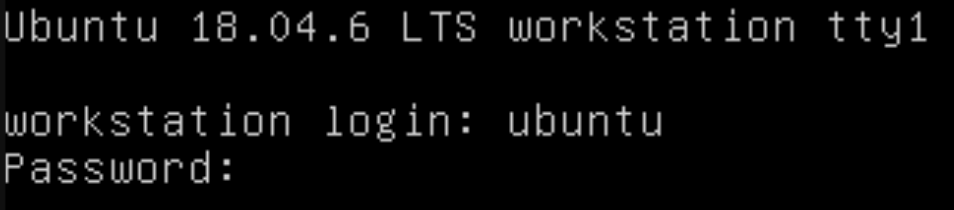
\includegraphics[width=\linewidth]{images/part1/step1.png}
        \end{center}
    \end{labstep}

    \begin{labstep}
        Launch the graphical user interface.
        \begin{lstlisting}
            ubuntu@workstation:~$ startx
        \end{lstlisting}

        \begin{center}
            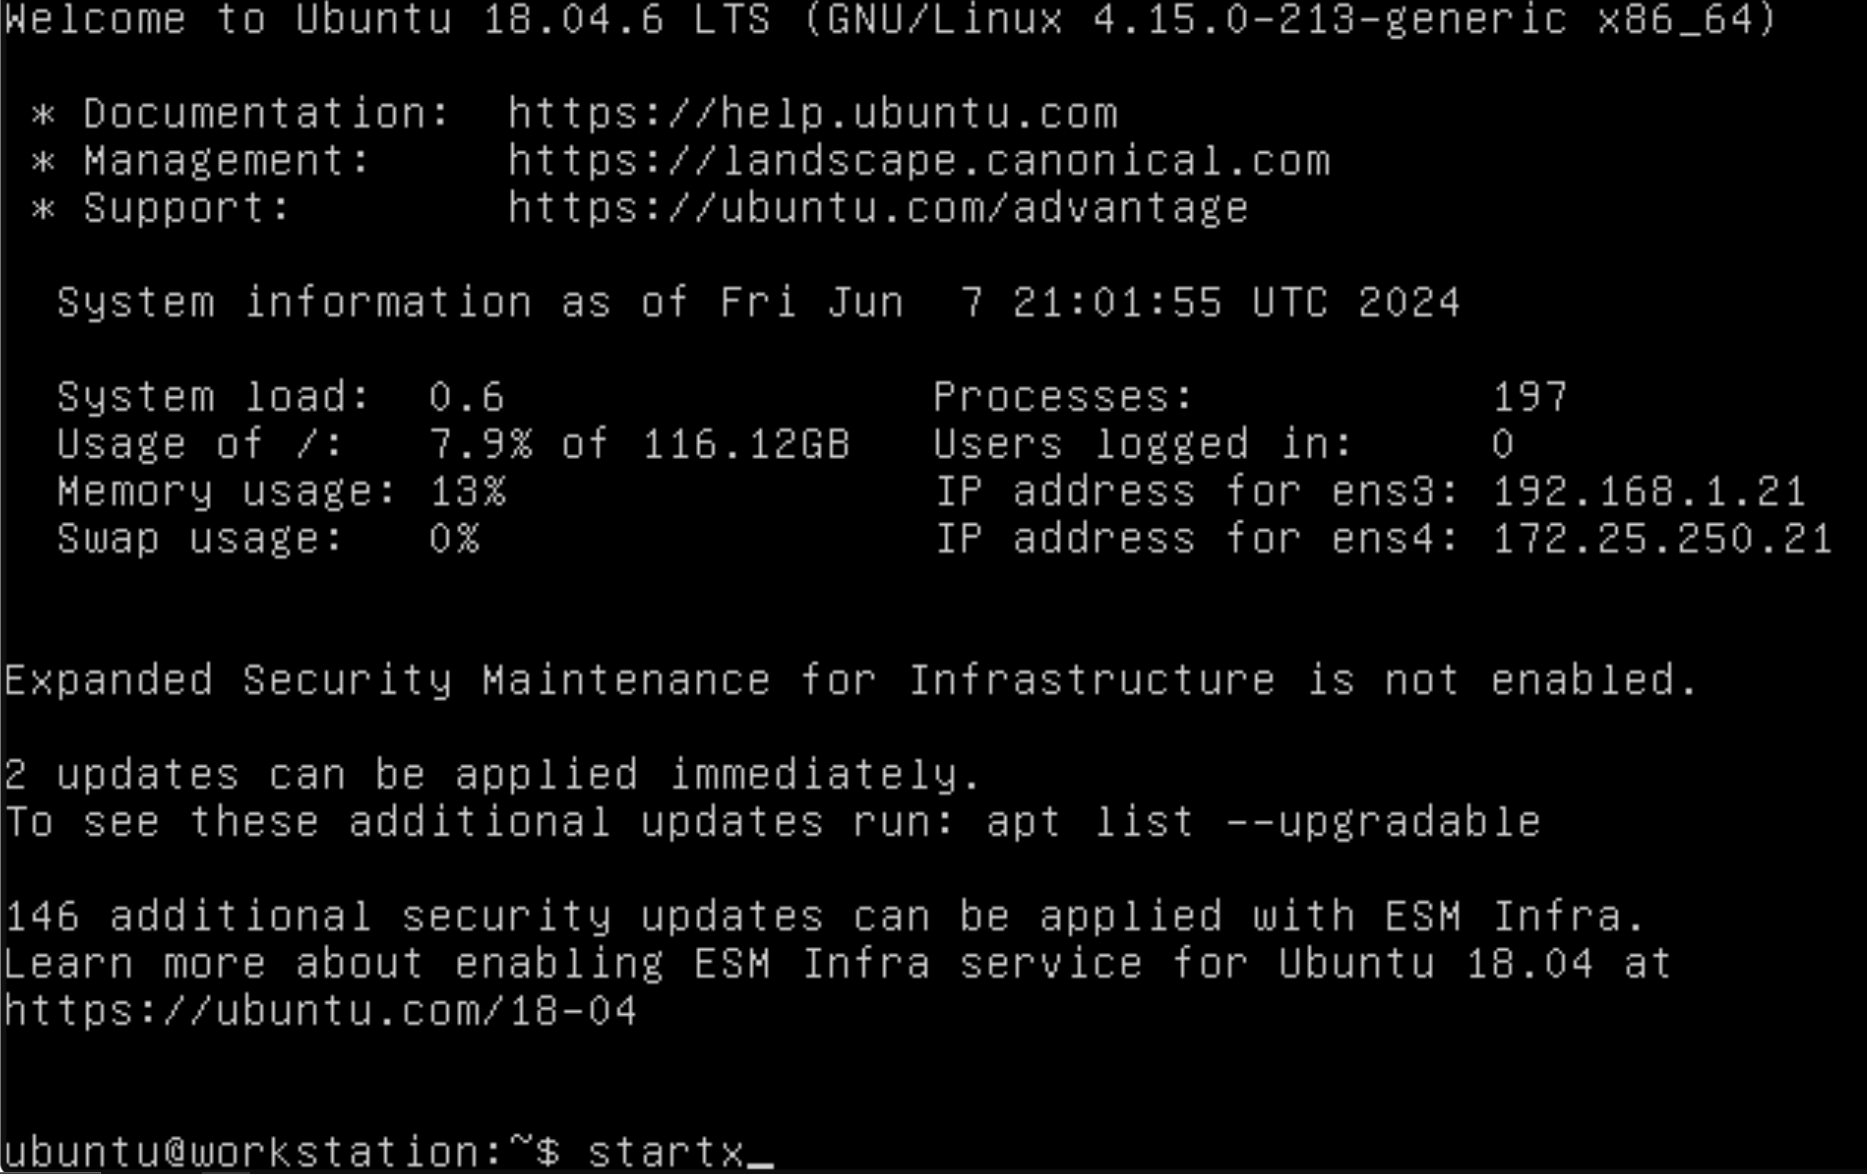
\includegraphics[width=\linewidth]{images/part1/step2.png}
        \end{center}
    \end{labstep}

    \begin{labstep}
        Open the web browser.

        \begin{center}
            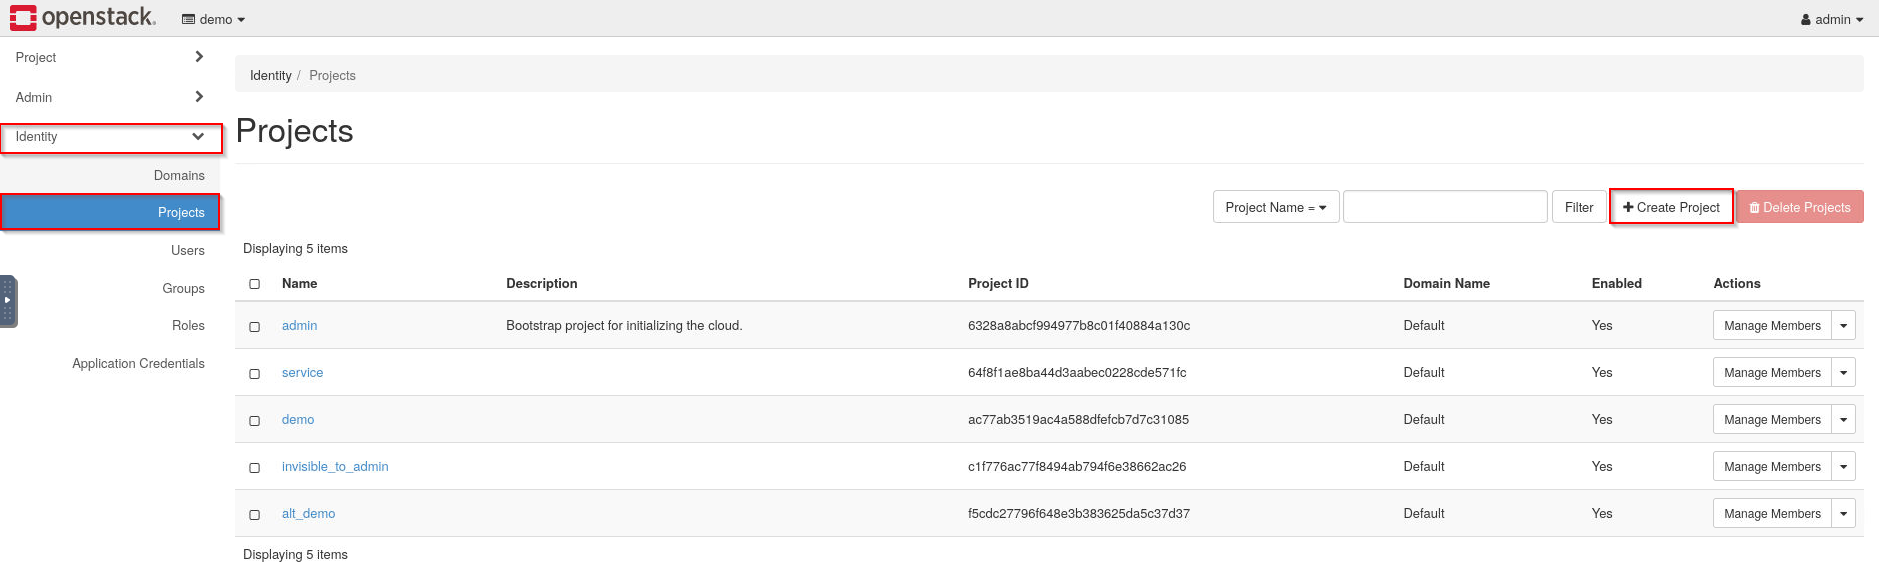
\includegraphics[scale=0.7]{images/part1/step3.png}
        \end{center}
    \end{labstep}

    \begin{labstep}
        Enter the IP address of the \textbf{devstack} machine (\textbf{192.168.1.20}) into the address bar, and log into the OpenStack Horizon Dashboard.
        The username is \textbf{admin}, and the password is \textbf{secret}.

        \begin{center}
            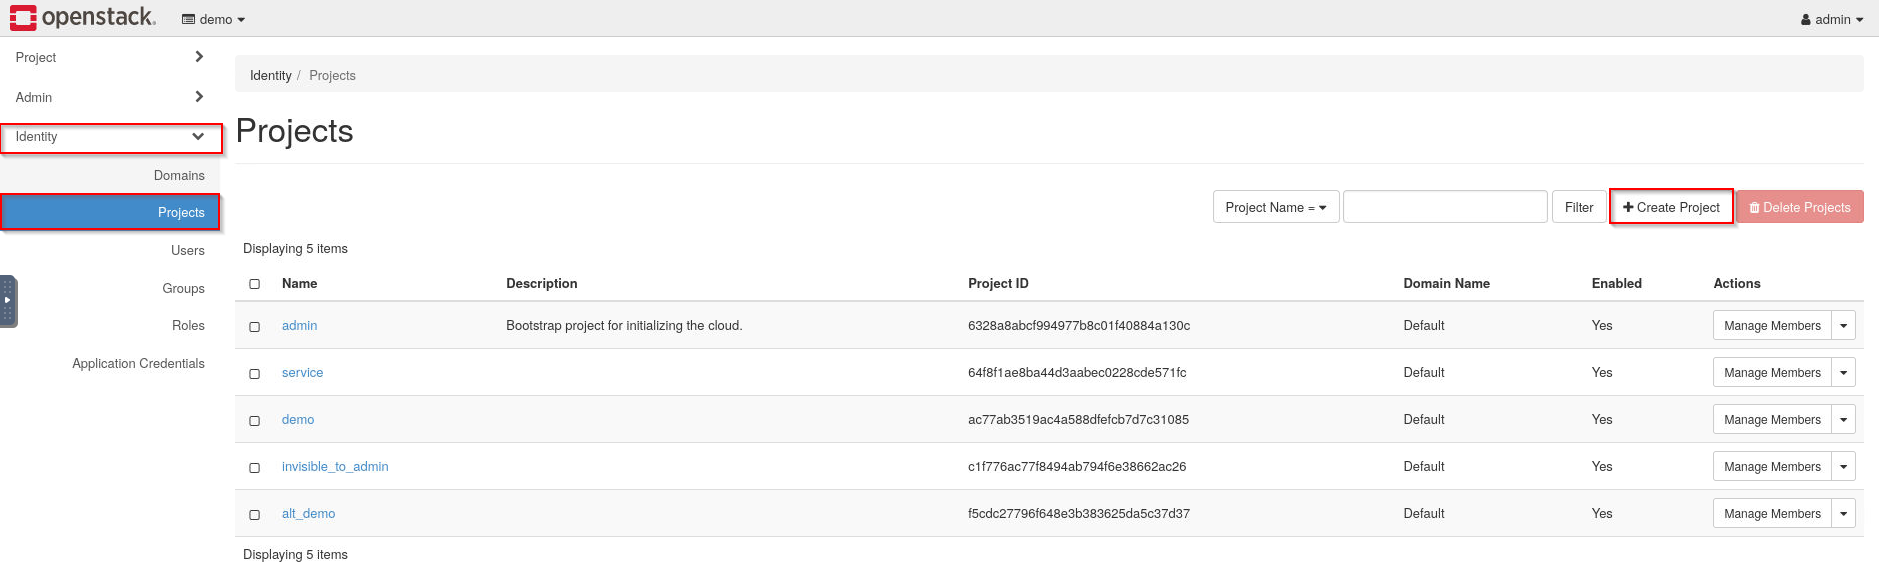
\includegraphics[scale=0.5]{images/part1/step4.png}
        \end{center}
    \end{labstep}

    \begin{labstep}
        Create a project named \textbf{dev}.
        First, navigate to \textbf{Identity $>$ Projects}, then click \textbf{Create Project}.

        \begin{center}
            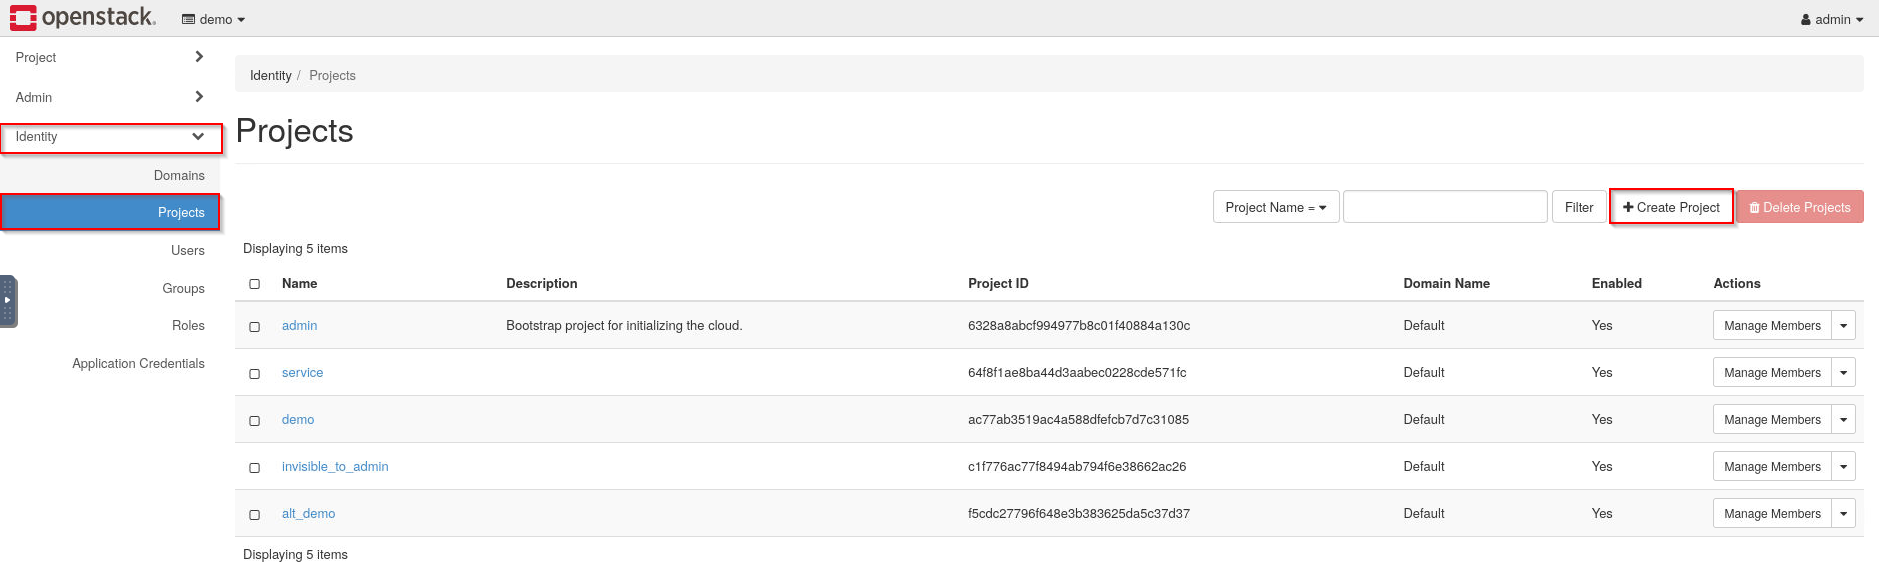
\includegraphics[width=\linewidth]{images/part1/step5.png}
        \end{center}
    \end{labstep}

    \begin{labstep}
        Enter \textbf{dev} in the \textit{Name} field and \textbf{Dev Project} in the \textit{Description} field.
        Click \textbf{Create Project}.

        \begin{center}
            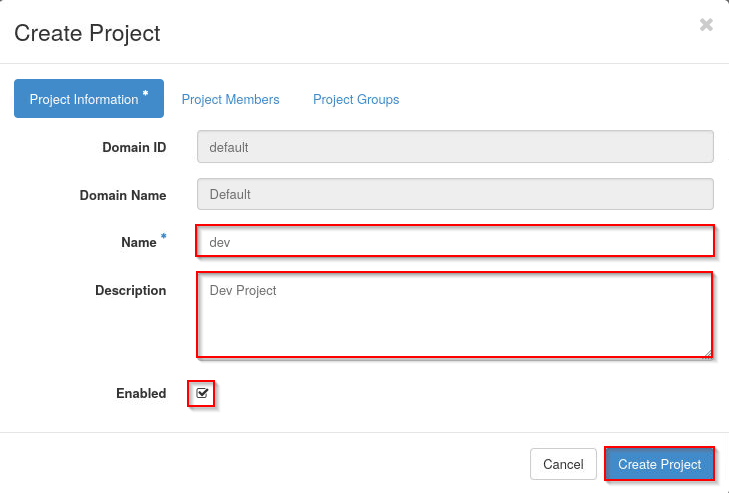
\includegraphics[width=\linewidth]{images/part1/step6.png}
        \end{center}
    \end{labstep}

    \begin{notebox}
        Notice the \textbf{dev} project now appears in the \textit{Horizon Dashboard}.
    \end{notebox}

    \begin{labstep}
        Suppose that the \textbf{alt\_demo} project is no longer needed and can be deleted.
        To delete this project, click the checkbox in the same row as \textbf{alt\_demo}, then click \textbf{Delete Projects}.

        \begin{center}
            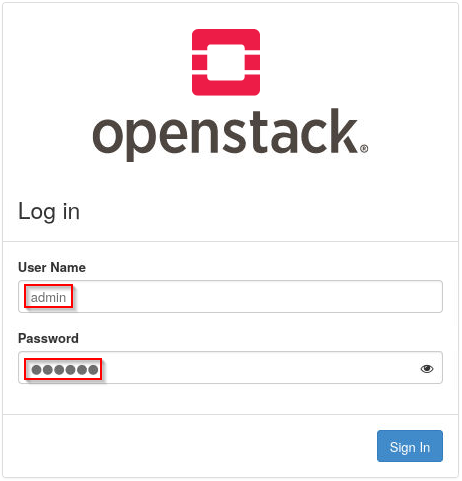
\includegraphics[width=\linewidth]{images/part1/step7.png}
        \end{center}
    \end{labstep}

    \begin{tipbox}
        The above method allows selecting and deleting multiple projects at once.
        A single project can also be deleted by clicking the dropdown in the same row as the project in the \textbf{Actions} column and clicking \textbf{Delete Project}.
    \end{tipbox}

    \begin{labstep}
        In the \textbf{Confirm Delete Projects} popup box, click \textbf{Delete Projects}.

        \begin{center}
            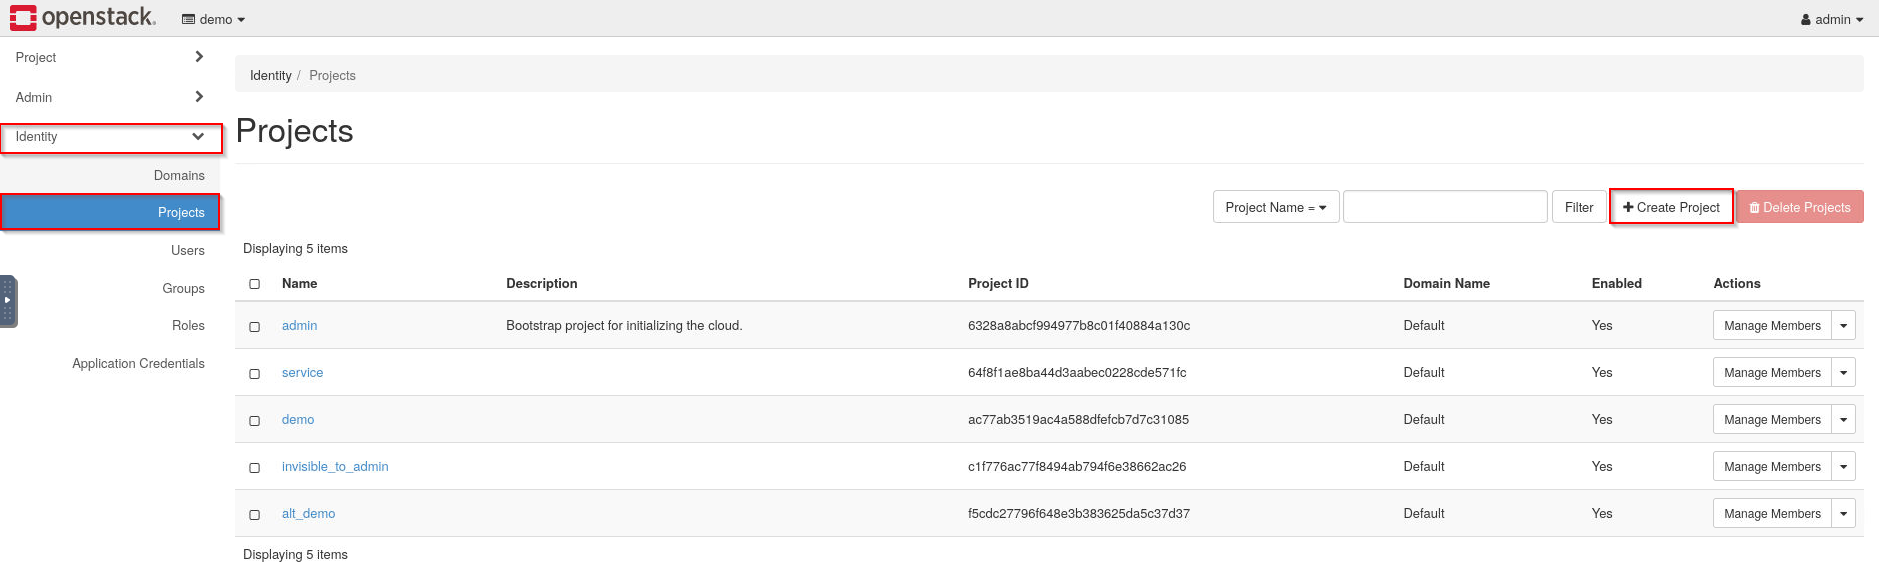
\includegraphics[width=\linewidth]{images/part1/step8.png}
        \end{center}
    \end{labstep}

    \begin{labstep}
        Log out of the Horizon Dashboard by clicking on the \textbf{admin} dropdown at the top right and selecting \textbf{Sign Out}.

        \begin{center}
            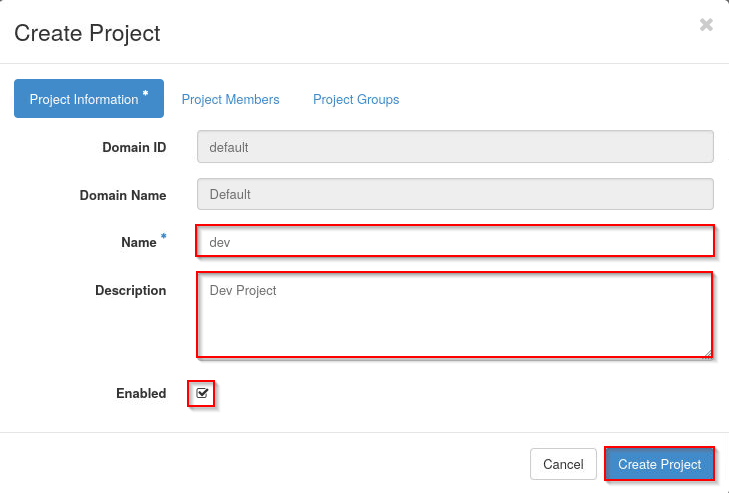
\includegraphics[scale=0.65]{images/part1/step9.png}
        \end{center}
    \end{labstep}

    \begin{labstep}
        Close the web browser and continue to the next task.
    \end{labstep}
\end{enumerate}

%%%%%%%%%%%
% Section 2
%%%%%%%%%%%
\section{Creating and Deleting Projects with the OpenStack Unified CLI}\label{sec:create_and_delete_projects_using_the_openstack_unified_cli}
In this task, you will use the \textit{OpenStack Unified CLI} to create and delete a project from the command line.

\begin{enumerate}
    \begin{labstep}
        Open a terminal by clicking the terminal icon in the icon bar at the bottom of the screen.
        A terminal can also be opened by right-clicking the desktop and selecting \textbf{Open Terminal Here}, or by selecting \textbf{Applications} at the top left of the screen, then selecting \textbf{Terminal Emulator}.

        \begin{center}
            
\includegraphics[width=\linewidth]{images/part2/step1.png}
        \end{center}
    \end{labstep}

    \begin{labstep}
        Use the \textbf{source} command with the \textbf{keystonerc-admin} argument to access OpenStack as the admin.
        \begin{lstlisting}
            ubuntu@workstation:~$ source ~/keystonerc-admin
        \end{lstlisting}

        \begin{center}
            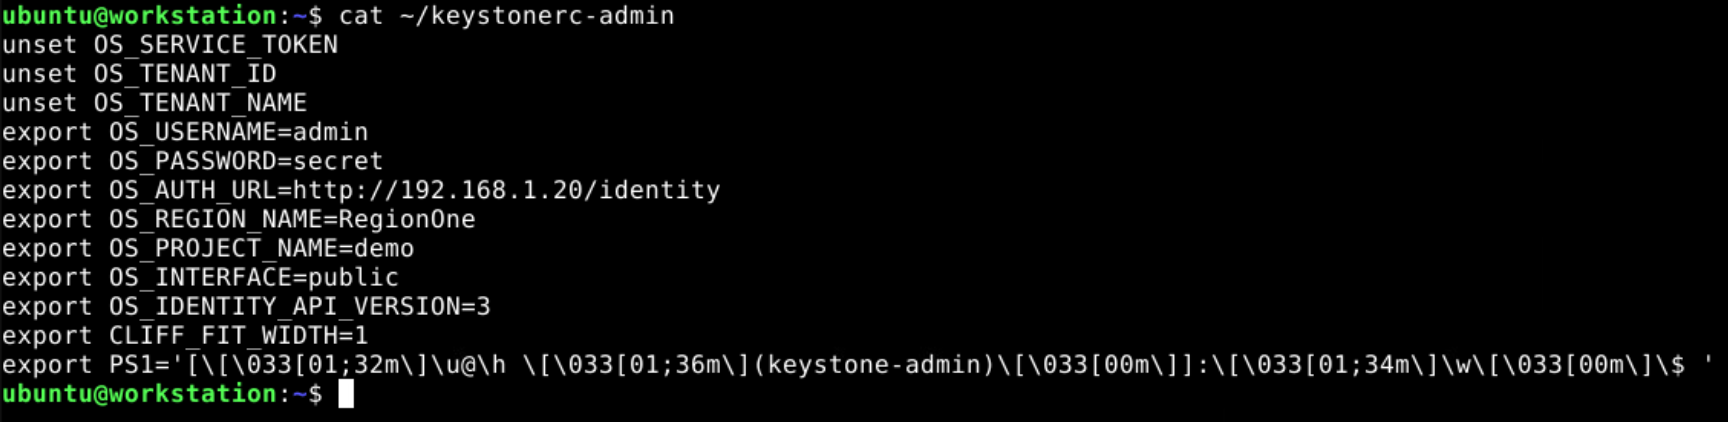
\includegraphics[width=\linewidth]{images/part2/step2.png}
        \end{center}
    \end{labstep}

    \begin{labstep}
        List the existing OpenStack projects.
        \begin{lstlisting}
            [ubuntu@workstation (keystone-admin)]:~$ openstack project list
        \end{lstlisting}

        \begin{center}
            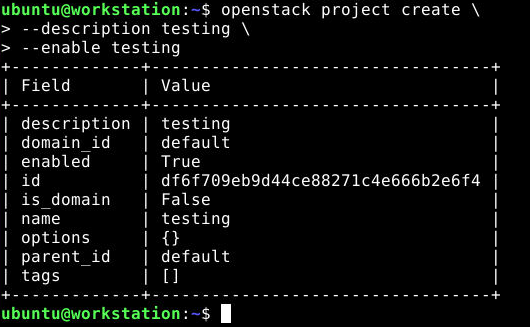
\includegraphics[width=\linewidth]{images/part2/step3.png}
        \end{center}
    \end{labstep}

    \begin{labstep}
        Create a project named \textbf{testing}.
        \begin{lstlisting}
            [ubuntu@workstation (keystone-admin)]:~$ openstack project create \
            > --description testing \
            > testing
        \end{lstlisting}

        \begin{center}
            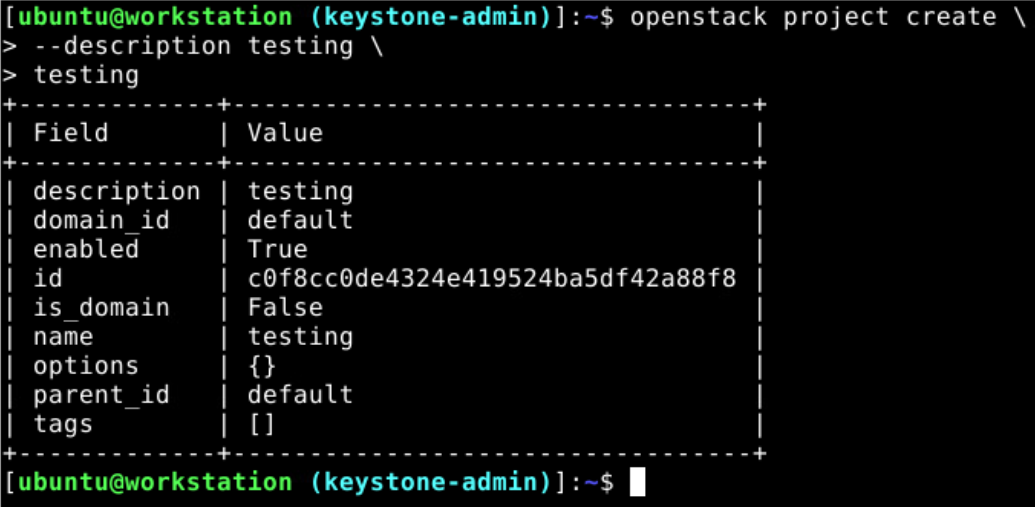
\includegraphics[width=\linewidth]{images/part2/step4.png}
        \end{center}
    \end{labstep}

    \begin{tipbox}
        When typing the command make sure there is a space between \textbf{create} and \textbf{\textbackslash}, and press \textbf{Enter} to get the \textbf{$>$} and continue typing the rest of the command.
    \end{tipbox}

    \begin{labstep}
        Verify that the project has been created.
        \begin{lstlisting}
            [ubuntu@workstation (keystone-admin)]:~$ openstack project list
        \end{lstlisting}

        \begin{center}
            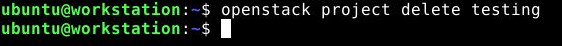
\includegraphics[width=\linewidth]{images/part2/step5.png}
        \end{center}
    \end{labstep}

    \begin{labstep}
        Show the project description that was adding during the creation of the project.
        \begin{lstlisting}
            [ubuntu@workstation (keystone-admin)]:~$ openstack project show testing
        \end{lstlisting}

        \begin{center}
            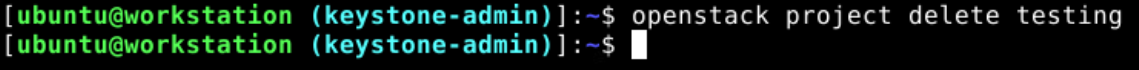
\includegraphics[width=\linewidth]{images/part2/step6.png}
        \end{center}
    \end{labstep}

    \begin{tipbox}
        The \textbf{openstack $<$object$>$ show} command prints the same information shown when the object was first created.
    \end{tipbox}

    \begin{labstep}
        The \textbf{dev} project from the previous step will be used throughout the remainder of the lab.
        The \textbf{testing} project was only created for demonstration and can be safely deleted.
        Delete the \textbf{testing} project.
        \begin{lstlisting}
            [ubuntu@workstation (keystone-admin)]:~$ openstack project delete testing
        \end{lstlisting}

        \begin{center}
            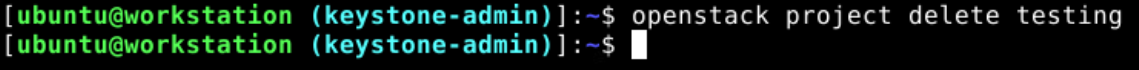
\includegraphics[width=\linewidth]{images/part2/step7.png}
        \end{center}
    \end{labstep}

    \begin{labstep}
        Verify that the \textbf{testing} project has been deleted by listing the projects again and noting that
        \textbf{testing} no longer appears.
        \begin{lstlisting}
            [ubuntu@workstation (keystone-admin)]:~$ openstack project list
        \end{lstlisting}

        \begin{center}
            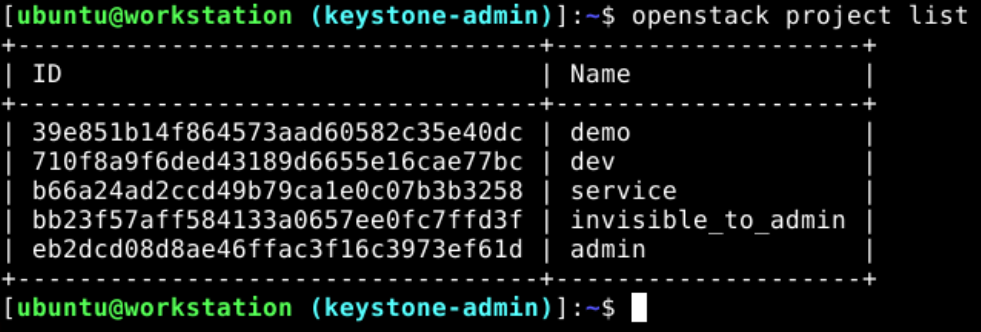
\includegraphics[width=\linewidth]{images/part2/step8.png}
        \end{center}
    \end{labstep}

    \begin{labstep}
        Leave the terminal window open and continue to the next task.
    \end{labstep}
\end{enumerate}

%%%%%%%%%%%
% Section 3
%%%%%%%%%%%
\section{Managing Users and Roles with the Horizon Dashboard}\label{sec:managing_users_using_the_horizon_dashboard}
In this task, you will use the \textit{Horizon Dashboard} to manage users, assign user roles, and configure user privileges.
You will create a user who is an administrator of the \textbf{dev} project, and that user will perform several admin actions in that project, such as creating user accounts, setting user passwords, and adding users to the project.

\begin{enumerate}
    \begin{labstep}
        Open the web browser, navigate to the OpenStack login page at \textbf{http://192.168.1.20}, and log in with the username \textbf{admin} and the password \textbf{secret}.

        \begin{center}
            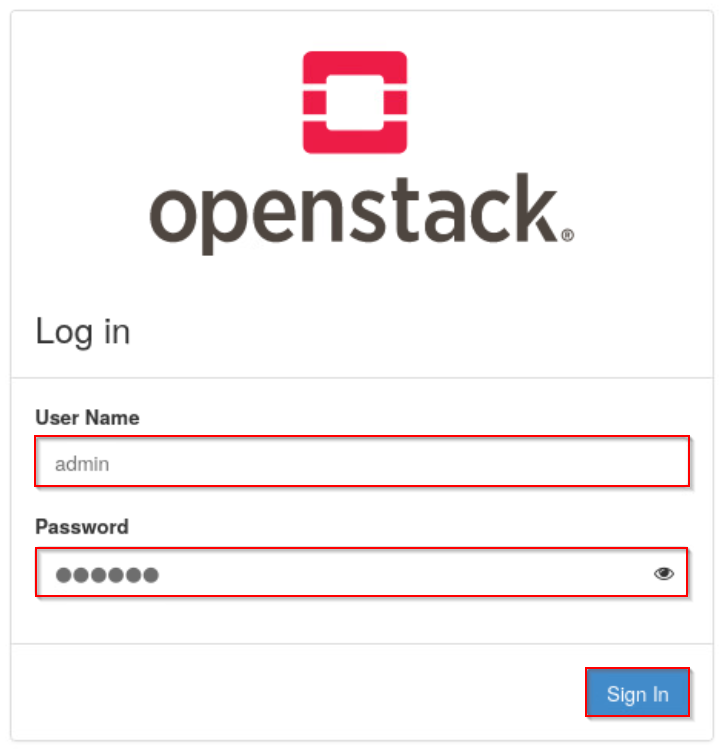
\includegraphics[scale=0.5]{images/part3/step1.png}
        \end{center}
    \end{labstep}

    \begin{labstep}
        Create the \textbf{cloud-admin} user with \textbf{admin} privileges in the \textbf{dev} project.
        This user will manage other users in the project and their roles.
        First, navigate to \textbf{Identity $>$ Users} and click \textbf{Create User}.

        \begin{center}
            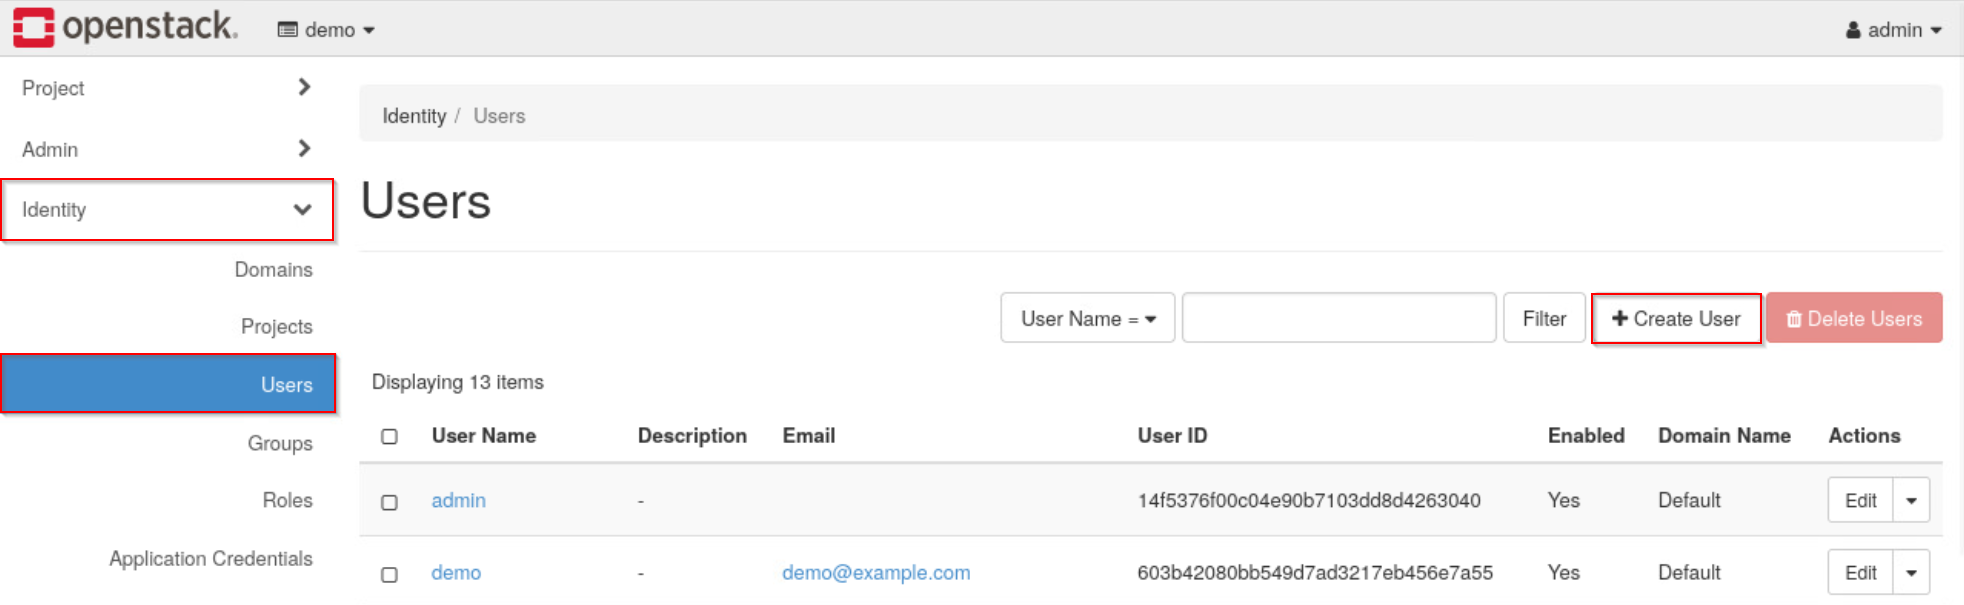
\includegraphics[width=\linewidth]{images/part3/step2.png}
        \end{center}
    \end{labstep}

    \begin{labstep}
        In the dialog box, enter \textbf{cloud-admin} in the \textit{User Name} field, and enter \textbf{secret} in the \textit{Password} and \textit{Confirm Password} fields.
        Select the \textbf{dev} project from the \textit{Primary Project} dropdown, and select \textbf{admin} in the \textit{Role} dropdown.
        Finally, leave the \textbf{Enabled} checkbox selected and click \textbf{Create User}.

        \begin{center}
            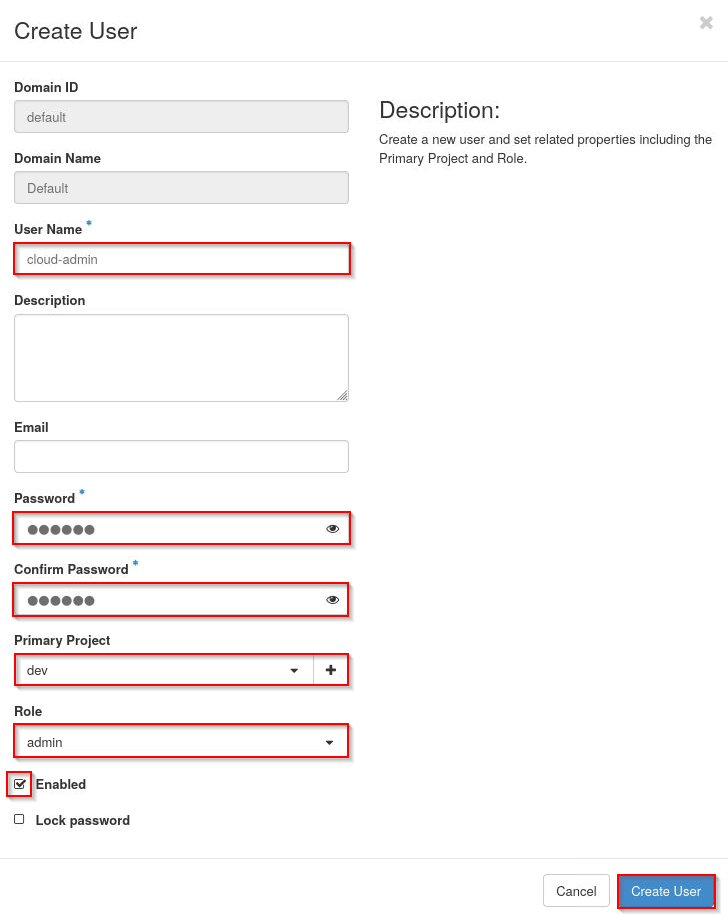
\includegraphics[scale=0.7]{images/part3/step3.png}
        \end{center}
    \end{labstep}

    \begin{tipbox}
        You may need to use the scroll bar on the right of the dialog to scroll down to see the projects and roles.
    \end{tipbox}

    \begin{labstep}
        Log out of the dashboard by clicking the \textbf{admin} dropdown in the top right corner, then clicking \textbf{Sign Out}, and log back in to the dashboard as the newly-created \textbf{cloud-admin} user with the password \textbf{secret}.
        Next, the \textbf{cloud-admin} user will create additional users and assign them to the \textbf{dev} project.

        \begin{center}
            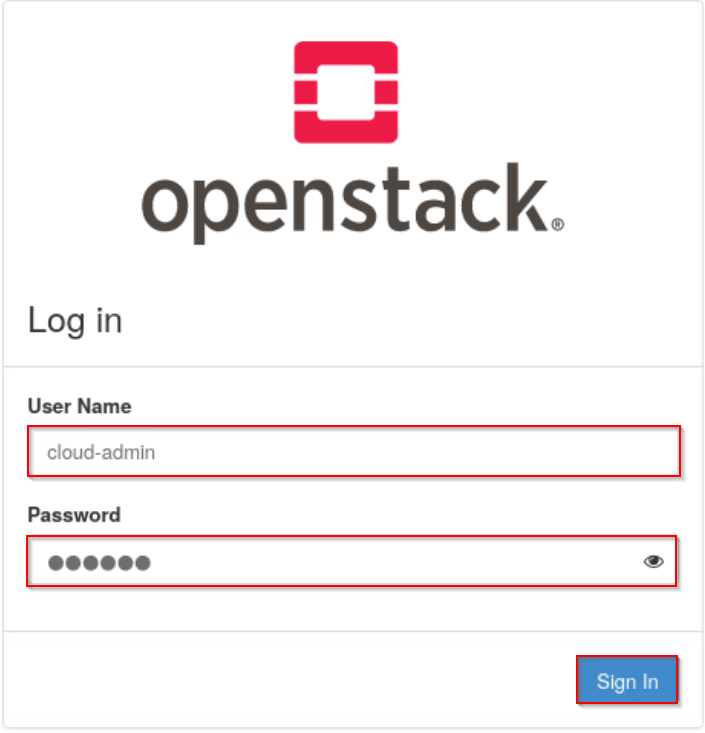
\includegraphics[scale=0.5]{images/part3/step4.png}
        \end{center}
    \end{labstep}

    \begin{labstep}\label{it:create-user-start}
        Navigate to \textbf{Identity $>$ Users} and click \textbf{Create User}.

        \begin{center}
            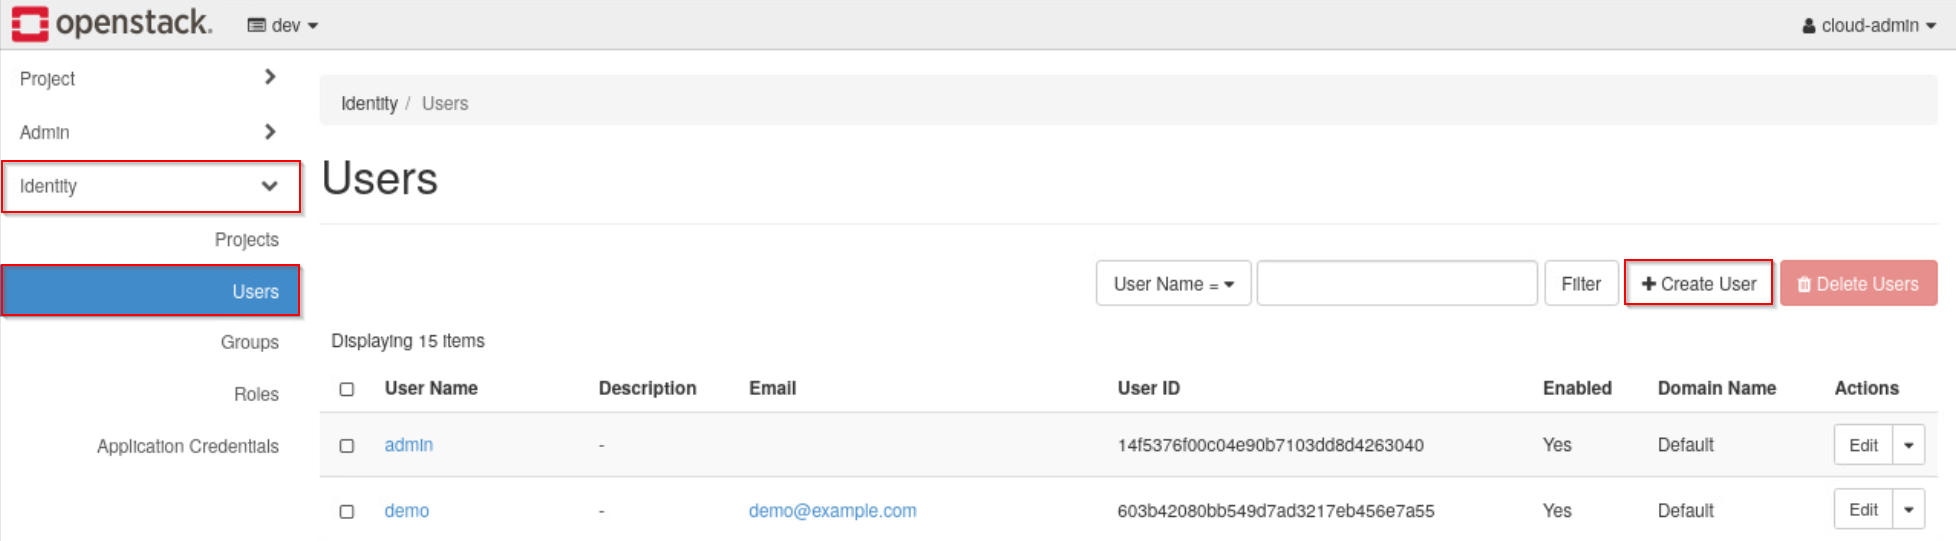
\includegraphics[width=\linewidth]{images/part3/step5.png}
        \end{center}
    \end{labstep}

    \begin{labstep}
        In the \textit{Create User} dialog box, enter \textbf{cloud-test1} in the \textit{User Name} field, and \textbf{secret} in the \textit{Password} and \textit{Confirm Password} fields.

        \begin{center}
            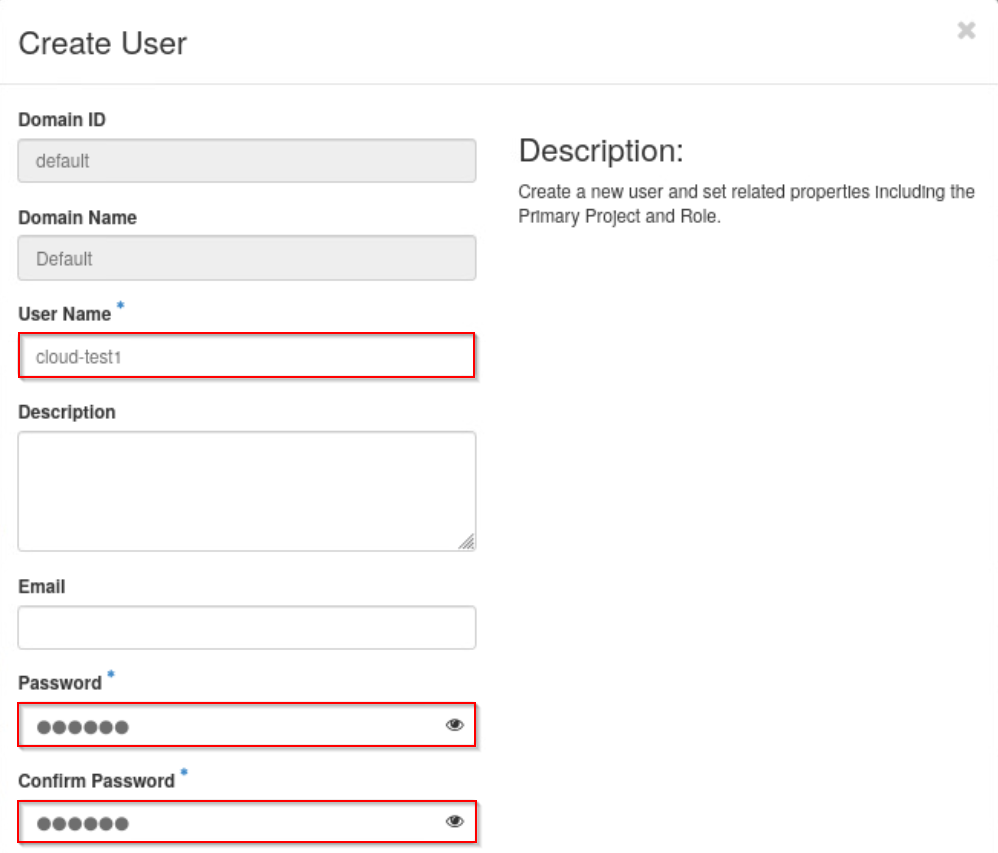
\includegraphics[width=\linewidth]{images/part3/step6.png}
        \end{center}
    \end{labstep}

    \begin{tipbox}
        You may need to use the scroll bar on the right side of the dialog box to see the rest of the fields.
    \end{tipbox}

    \begin{labstep}\label{it:create-user-end}
        After scrolling down if necessary, select the \textbf{dev} project from the \textit{Primary Project} dropdown.
        Leave the \textit{Role} set to \textbf{member}.
        Click \textbf{Create User}.

        \begin{center}
            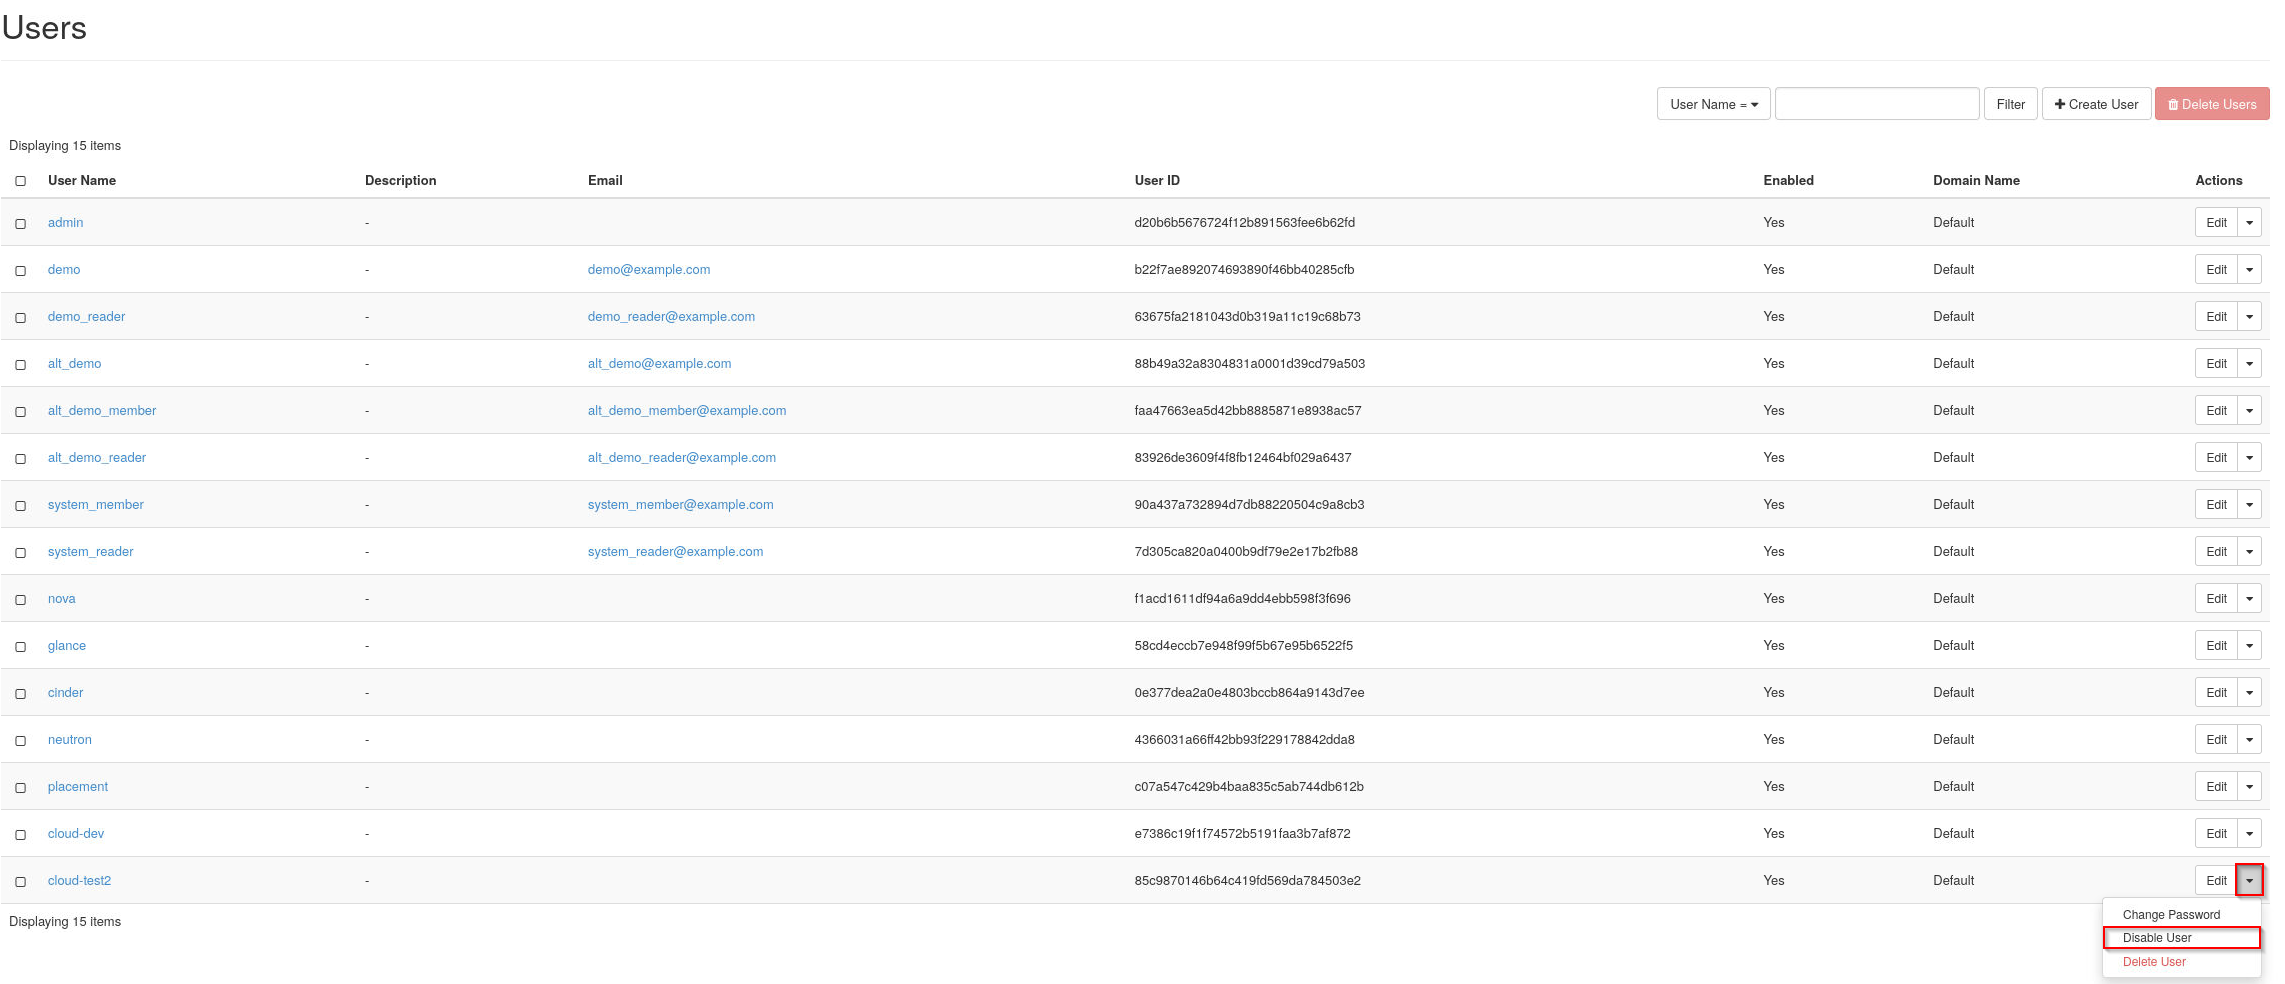
\includegraphics[width=\linewidth]{images/part3/step7.png}
        \end{center}
    \end{labstep}

    \begin{labstep}
        Repeat steps~\ref{it:create-user-start} through~\ref{it:create-user-end} to create the \textbf{cloud-test2} user account.
    \end{labstep}

    \begin{labstep}
        Delete the \textbf{cloud-test1} user account.
        On the \textit{Users} tab, click the dropdown in the \textit{Actions} column in the row for the \textbf{cloud-test1} user account.
        Click \textbf{Delete User}, and confirm the deletion in the popup box that appears.

        \begin{center}
            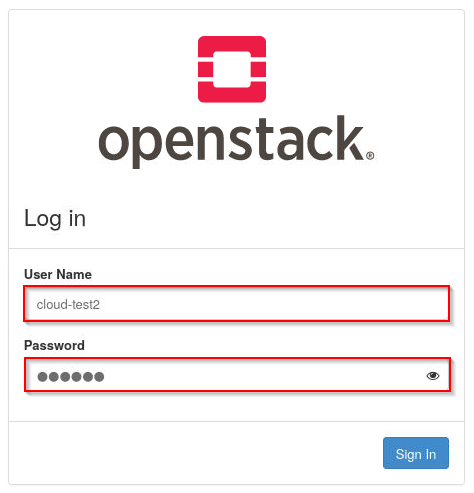
\includegraphics[width=\linewidth]{images/part3/step9.png}
        \end{center}
    \end{labstep}

    \begin{tipbox}
        To delete multiple users at once, select the checkboxes beside the users to be deleted, and click \textbf{Delete Users} at the top right of the page.
    \end{tipbox}

    \begin{labstep}
        Next, we will disable the \textbf{cloud-test2} user, which does not allow that user to log in.
        To show that the user is currently enabled and able to log in, first log out of the dashboard.
        Then, log back in with the username \textbf{cloud-test2} and the password \textbf{secret}.

        \begin{center}
            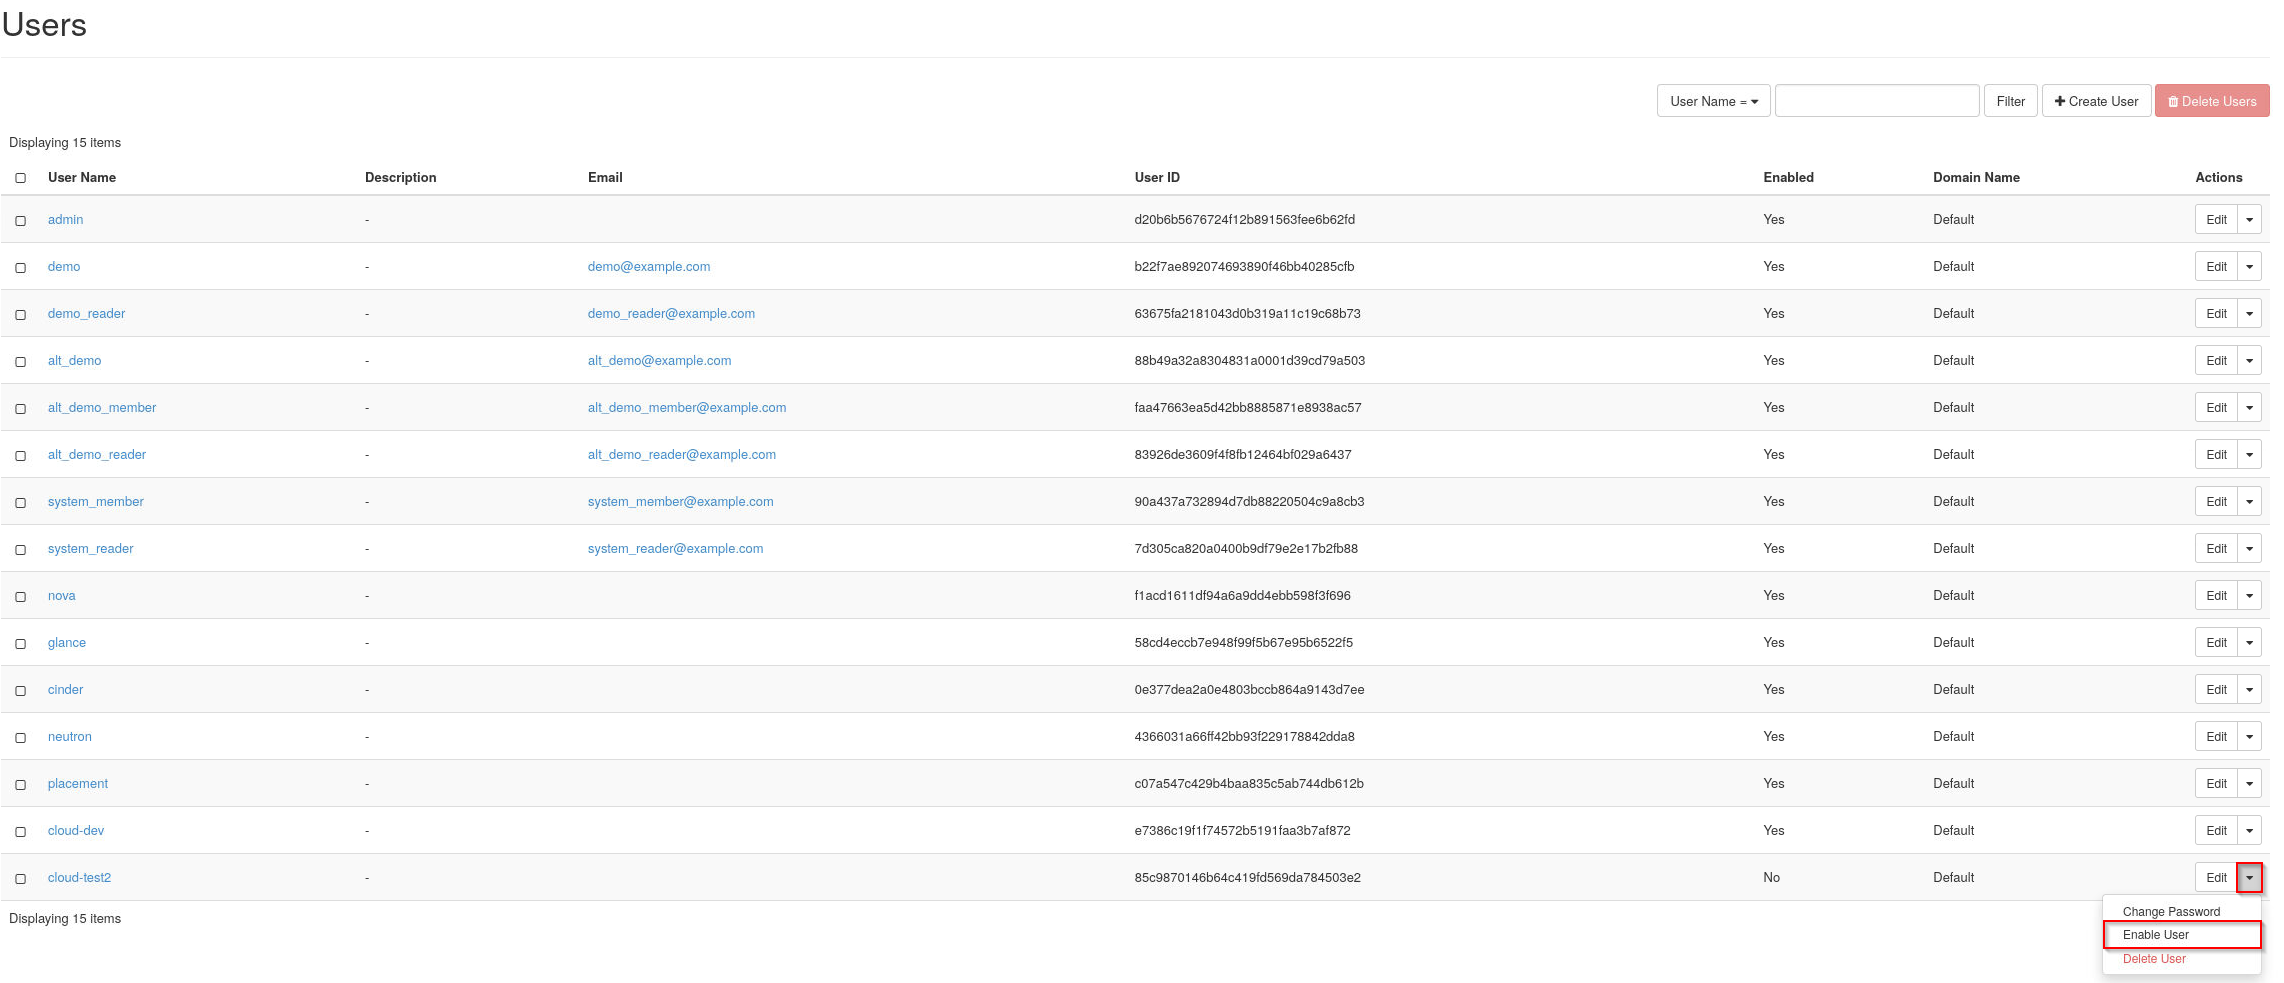
\includegraphics[scale=0.5]{images/part3/step10.png}
        \end{center}
    \end{labstep}

    \begin{labstep}
        Since the user is able to log in, it is enabled.
        For further proof, navigate to \textbf{Identity $>$ Users} and note that the list of users is visible.

        \begin{center}
            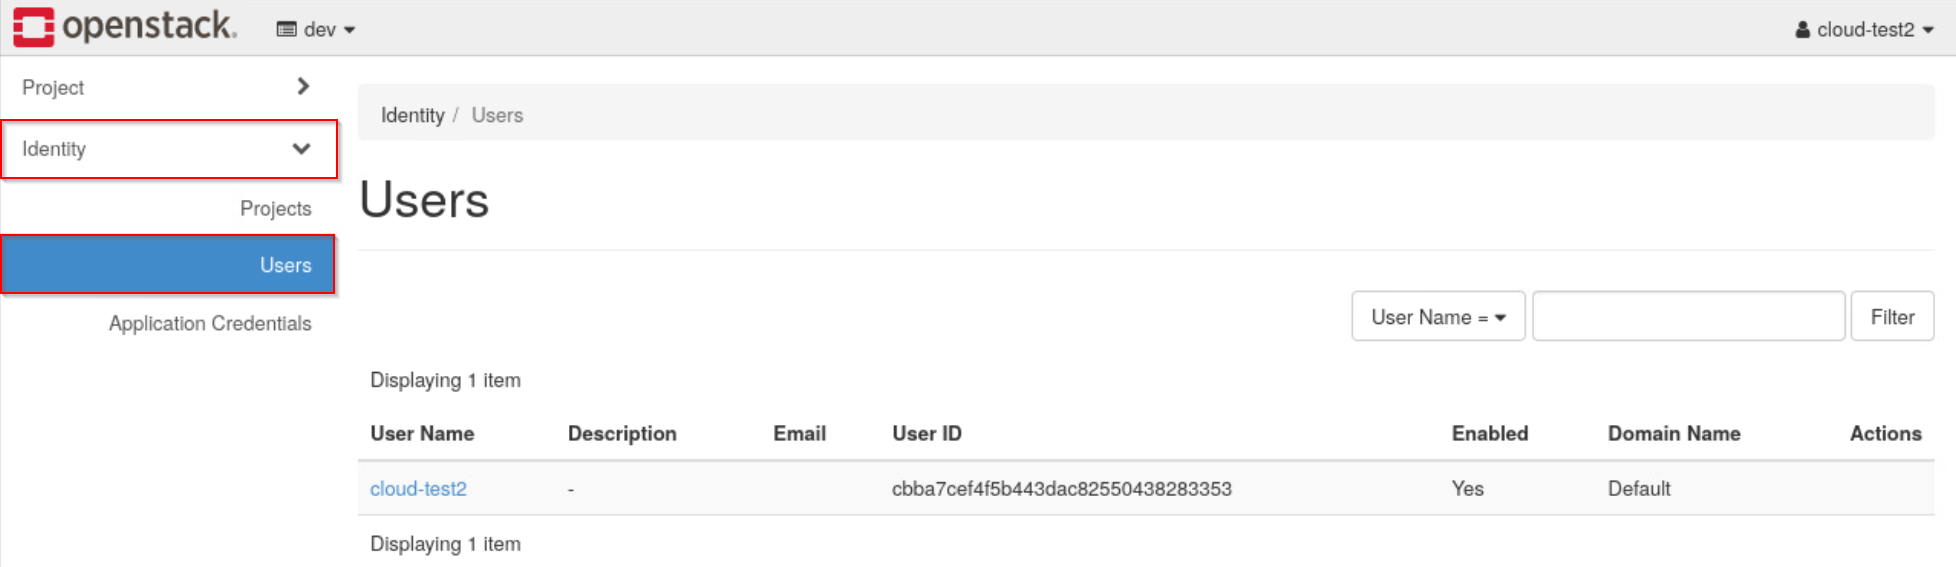
\includegraphics[width=\linewidth]{images/part3/step11.png}
        \end{center}
    \end{labstep}

    \begin{notebox}
        Notice, also, that since \textbf{cloud-test2} has only member privileges, it cannot see other users, even other members of the \textbf{dev} project.
        Additionally, this user cannot see the \textbf{Admin} tab in the sidebar.
    \end{notebox}

    \begin{labstep}
        Log out of the dashboard, and log back in with the username \textbf{cloud-admin} and the password \textbf{secret}.

        \begin{center}
            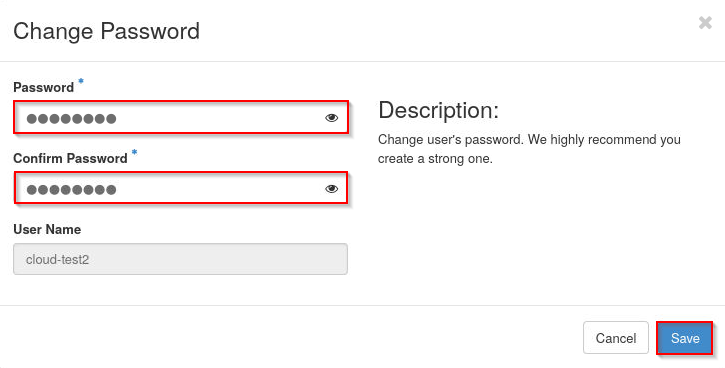
\includegraphics[scale=0.5]{images/part3/step12.png}
        \end{center}
    \end{labstep}

    \begin{labstep}
        Navigate to \textbf{Identity $>$ Users}.
        Disable the \textbf{cloud-test2} user account.
        On the \textit{Users} tab, click the dropdown in the \textit{Actions} column for the \textbf{cloud-test2} user account entry, and click \textbf{Disable User}.

        \begin{center}
            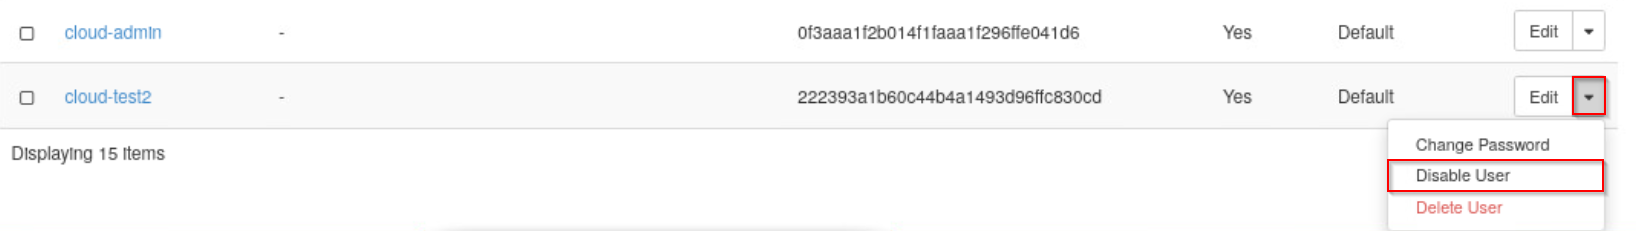
\includegraphics[width=\linewidth]{images/part3/step13.png}
        \end{center}
    \end{labstep}

    \begin{labstep}
        Log out one more time, and attempt to log in as \textbf{cloud-test2} with the password \textbf{secret}.

        \begin{center}
            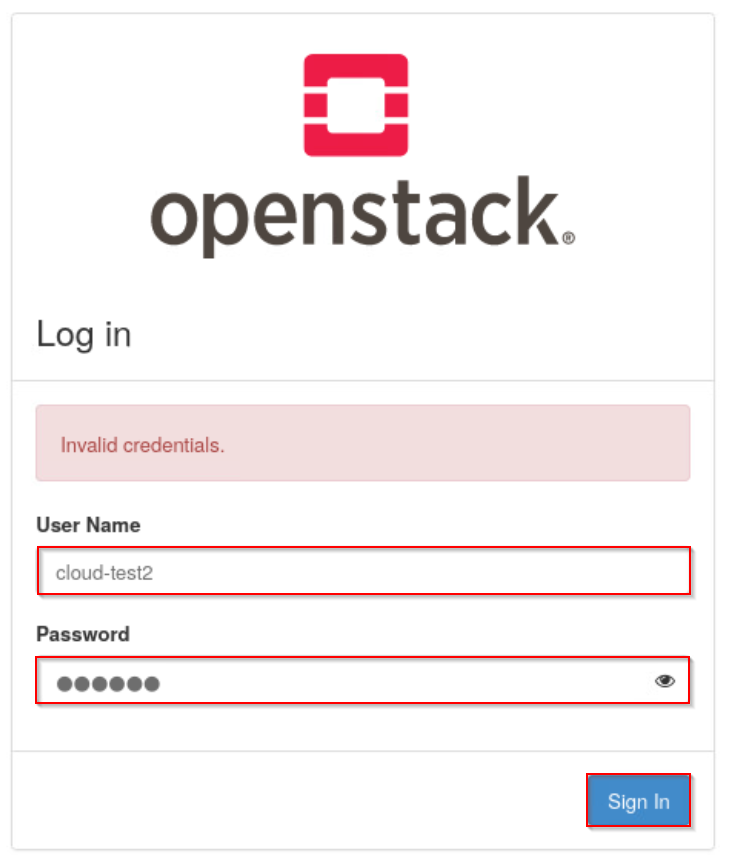
\includegraphics[scale=0.5]{images/part3/step14.png}
        \end{center}
    \end{labstep}

    \begin{notebox}
        The account is now disabled, and the \textbf{cloud-test2} user will receive an invalid credentials error when it attempts to log in.
    \end{notebox}

    \begin{labstep}
        Log back in to the dashboard as \textbf{cloud-admin} with the password \textbf{secret}.
        Navigate to \textbf{Identity $>$ Users}.
        Click the dropdown in the \textit{Actions} column in the row for \textbf{cloud-test2}, and click \textbf{Change Password}.

        \begin{center}
            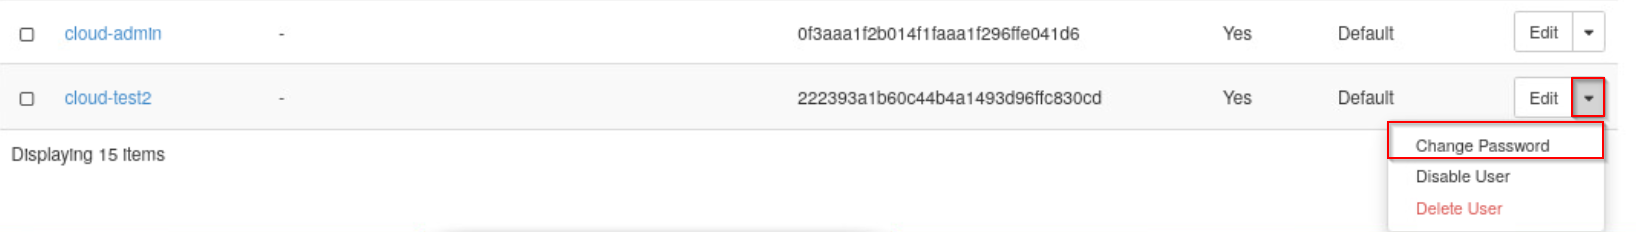
\includegraphics[width=\linewidth]{images/part3/step15.png}
        \end{center}
    \end{labstep}

    \begin{labstep}
        Change the password for \textbf{cloud-test2} to \textbf{password}.
        Enter \textbf{password} into the
        \textit{Password} and \textit{Confirm Password} fields, then click \textbf{Save}.

        \begin{center}
            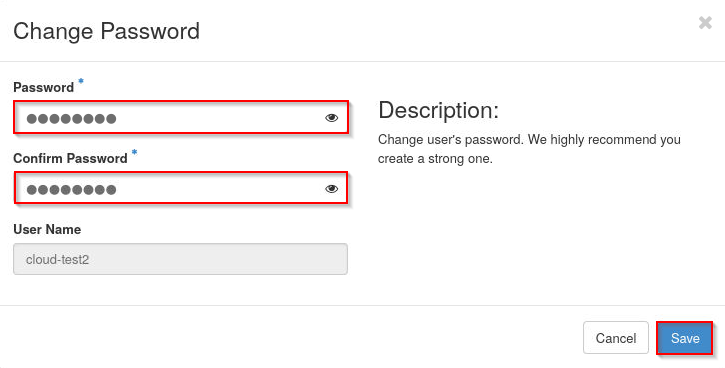
\includegraphics[width=\linewidth]{images/part3/step16.png}
        \end{center}
    \end{labstep}

    \begin{labstep}
        Back on the \textbf{Users} page, click the same dropdown as before, and click \textbf{Enable User} to allow \textbf{cloud-test2} to log in and perform actions.

        \begin{center}
            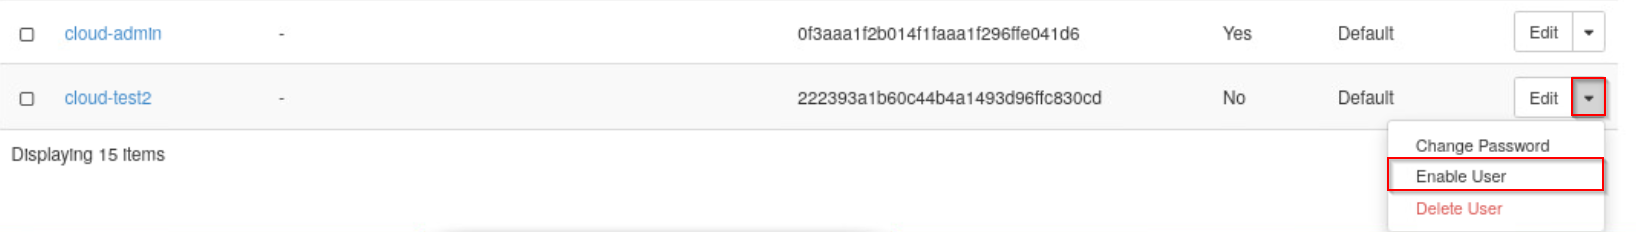
\includegraphics[width=\linewidth]{images/part3/step17.png}
        \end{center}
    \end{labstep}

    \begin{labstep}
        Log out of the dashboard and log back in as \textbf{cloud-test2} with the password \textbf{password} to verify that the user's password has been set and that the user can log in.

        \begin{center}
            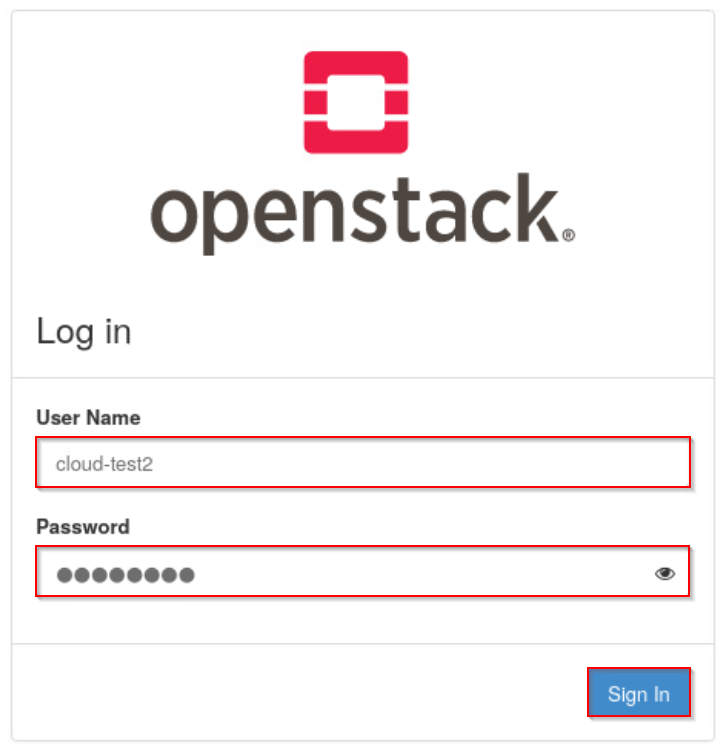
\includegraphics[scale=0.5]{images/part3/step18.png}
        \end{center}
    \end{labstep}

    \begin{notebox}
        The \textbf{cloud-test2} and \textbf{cloud-test3} users were not deleted in this section because they will be used in the following section to demonstrate deleting users from the command line.
    \end{notebox}

    \begin{labstep}
        Log out of the dashboard and close the web browser.
        Continue to the next task.
    \end{labstep}
\end{enumerate}

%%%%%%%%%%%
% Section 4
%%%%%%%%%%%
\section{Managing Users and Roles with the OpenStack Unified CLI}\label{sec:managing_users_using_the_openstack_unified_cli}
In this task, you will use the \textit{OpenStack Unified CLI} to manage users, assign user roles, and configure user privileges.

\begin{enumerate}
    \begin{labstep}
        Open a terminal if you do not already have one running, and navigate to the home directory.
    \end{labstep}

    \begin{labstep}
        Before sourcing any credentials, let us take a closer look at the keystone credentials file we have been using up to this point.
        We have not yet looked at the details of this file, but they will become relevant in this section.
        The \textbf{keystonerc-admin} file in the home directory defines several \textbf{OS\_*} environment variables that allow you to use the OpenStack platform on the \textbf{devstack} server through the OpenStack Unified CLI.
        You can run \textbf{cat} on the file to view its contents.
        The file lists the username as \textbf{admin}, the password as \textbf{secret}, and the project as \textbf{demo}.
        The address for \textbf{OS\_AUTH\_URL} is the IP address of the \textbf{devstack} server, \textbf{192.168.1.20}.
        \begin{lstlisting}
            ubuntu@workstation:~$ cat ~/keystonerc-admin
        \end{lstlisting}

        \begin{center}
            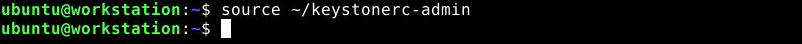
\includegraphics[width=\linewidth]{images/part4/step2.png}
        \end{center}
    \end{labstep}

    \begin{notebox}
        When the \textbf{source} command is used on a keystone credentials file, it enables all the \textbf{OS\_*} environment variables included in the file.
    \end{notebox}

    \begin{notebox}
        The \textbf{export PS1=…} line at the end of the keystone credentials file modifies the shell prompt to show the OpenStack user whose credentials are keyed in.
    \end{notebox}

    \begin{notebox}
        The same prompt without color can be achieved with the line \textbf{export PS1='[\textbackslash u@\textbackslash h (keystone-admin)]:\textbackslash w\$ '}.
        Here, \textbf{\textbackslash u} stands for the current username, \textbf{\textbackslash h} is the hostname, and \textbf{\textbackslash w} is the current working directory.
        The other escape sequences specify the colors of the prompt.
        For example, \textbf{\textbackslash[\textbackslash 033[01;32m\textbackslash]} sets the color to a light green, and \textbf{\textbackslash[\textbackslash 033[00m\textbackslash]} resets the color to the default (white in this case).
    \end{notebox}

    \begin{labstep}
        Source the credentials for \textbf{admin} from the \textbf{keystonerc-admin} file.
        \begin{lstlisting}
            ubuntu@workstation:~$ source ~/keystonerc-admin
        \end{lstlisting}

        \begin{center}
            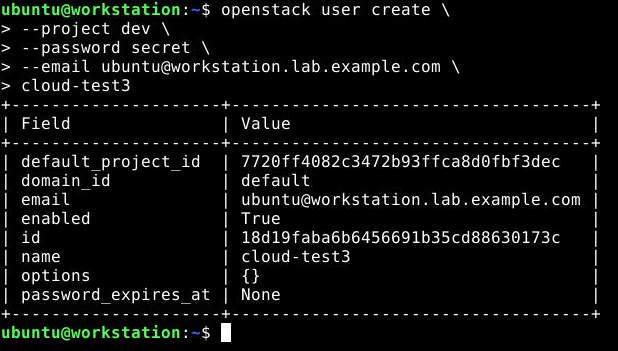
\includegraphics[width=\linewidth]{images/part4/step3.png}
        \end{center}
    \end{labstep}

    \begin{labstep}
        Verify that the \textbf{OS\_*} environment variables have been exported to the shell environment.
        \begin{lstlisting}
            [ubuntu@workstation (keystone-admin)]:~$ env | grep OS_
        \end{lstlisting}

        \begin{center}
            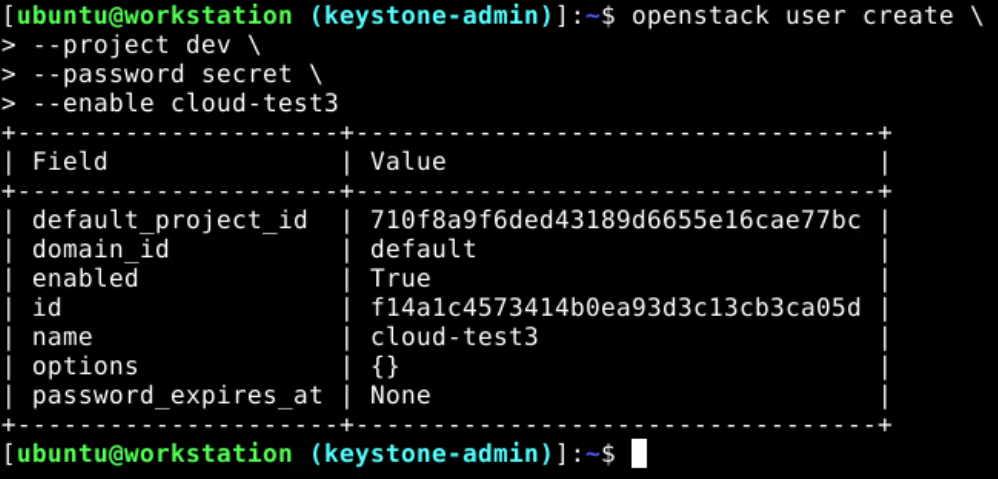
\includegraphics[width=\linewidth]{images/part4/step4.png}
        \end{center}
    \end{labstep}

    \begin{labstep}
        With a better grasp of the keystone credentials file, we can proceed to managing users.
        First, list the existing OpenStack users.
        \begin{lstlisting}
            [ubuntu@workstation (keystone-admin)]:~$ openstack user list
        \end{lstlisting}

        \begin{center}
            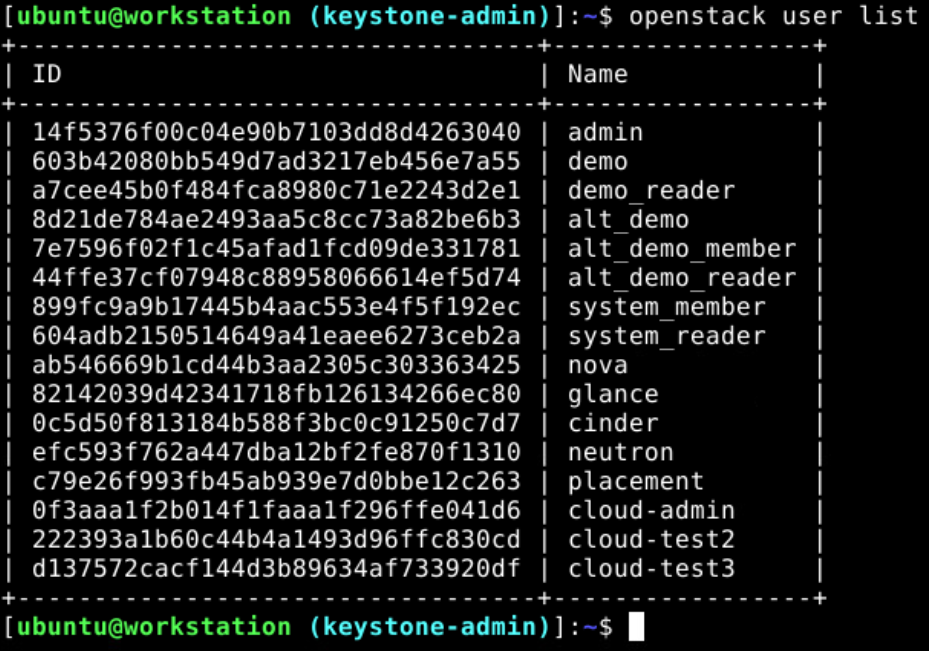
\includegraphics[width=\linewidth]{images/part4/step5.png}
        \end{center}
    \end{labstep}

    \begin{labstep}
        A user must have sufficient privileges to create roles and assign them to other users.
        The current user, \textbf{admin} has full administrator privileges and can create and assign roles to any user.
        Create the \textbf{cloud-test3} user on the \textbf{dev} project with the password \textbf{secret}.
        \begin{lstlisting}
            [ubuntu@workstation (keystone-admin)]:~$ openstack user create \
            > --project dev \
            > --password secret \
            > cloud-test3
        \end{lstlisting}

        \begin{center}
            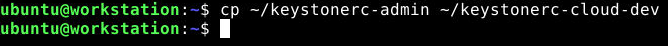
\includegraphics[width=\linewidth]{images/part4/step6.png}
        \end{center}
    \end{labstep}

    \begin{labstep}
        Verify that the user was created.
        \begin{lstlisting}
            [ubuntu@workstation (keystone-admin)]:~$ openstack user list
        \end{lstlisting}

        \begin{center}
            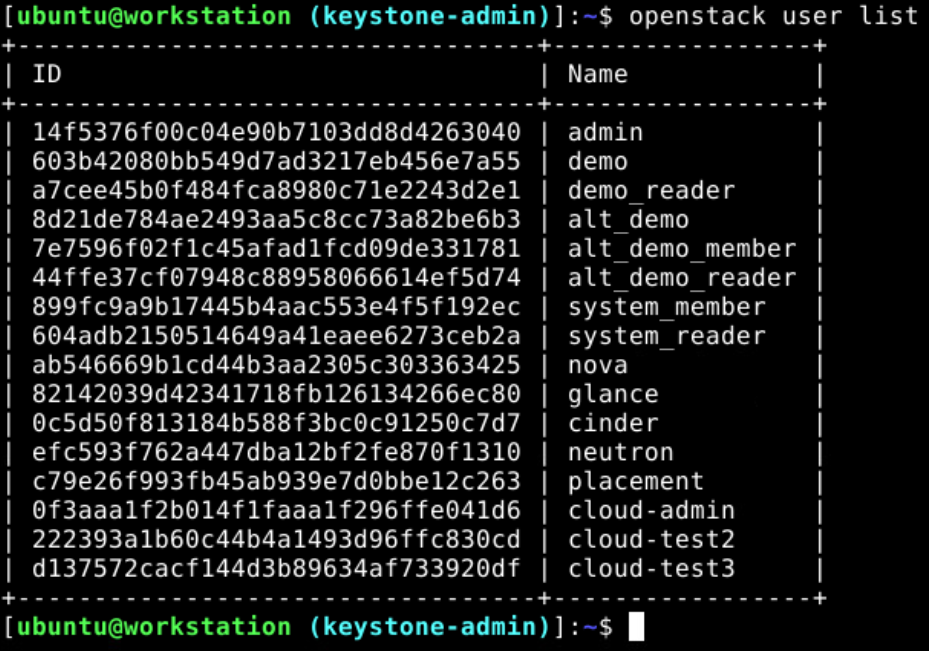
\includegraphics[width=\linewidth]{images/part4/step7.png}
        \end{center}
    \end{labstep}

    \begin{tipbox}
        When searching for a particular value in a long list, it is often helpful to pipe the command's output to \textbf{grep} or another string searching tool.
        For example, this command would show only the line containing \textbf{cloud-test3}:
        \begin{lstlisting}
            [ubuntu@workstation (keystone-admin)]:~$ openstack user list | \
            > grep cloud-test3
        \end{lstlisting}
        However, these labs will almost always show the full output of the \textbf{list} commands to show a snapshot of what the current state should be as you follow the instructions.
    \end{tipbox}

    \begin{labstep}

        When created through the OpenStack Unified CLI, users are not automatically assigned a role, and there is no option to assign a role in the \textbf{openstack user create} command.
        This is because roles are scoped to projects, not to users.
        Therefore, the \textbf{cloud-test3} user will need to be assigned a role on the \textbf{dev} project before being able to perform any actions within it.
        List the available roles to choose an appropriate one.
        \begin{lstlisting}
            [ubuntu@workstation (keystone-admin)]:~$ openstack role list
        \end{lstlisting}

        \begin{center}
            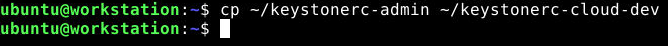
\includegraphics[width=\linewidth]{images/part4/step8.png}
        \end{center}
    \end{labstep}

    \begin{tipbox}
        To verify that a user is not assigned a role by default, you can run the following command and note the empty output:
        \begin{lstlisting}
            [ubuntu@workstation (keystone-admin)]:~$ openstack role list assignment list \
            > --user cloud-test3
        \end{lstlisting}
    \end{tipbox}

    \begin{labstep}
        Assign \textbf{cloud-test3} the \textbf{member} role on the \textbf{dev} project.
        \begin{lstlisting}
            [ubuntu@workstation (keystone-admin)]:~$ openstack role add \
            > --project dev \
            > --user cloud-test3 \
            > member
        \end{lstlisting}

        \begin{center}
            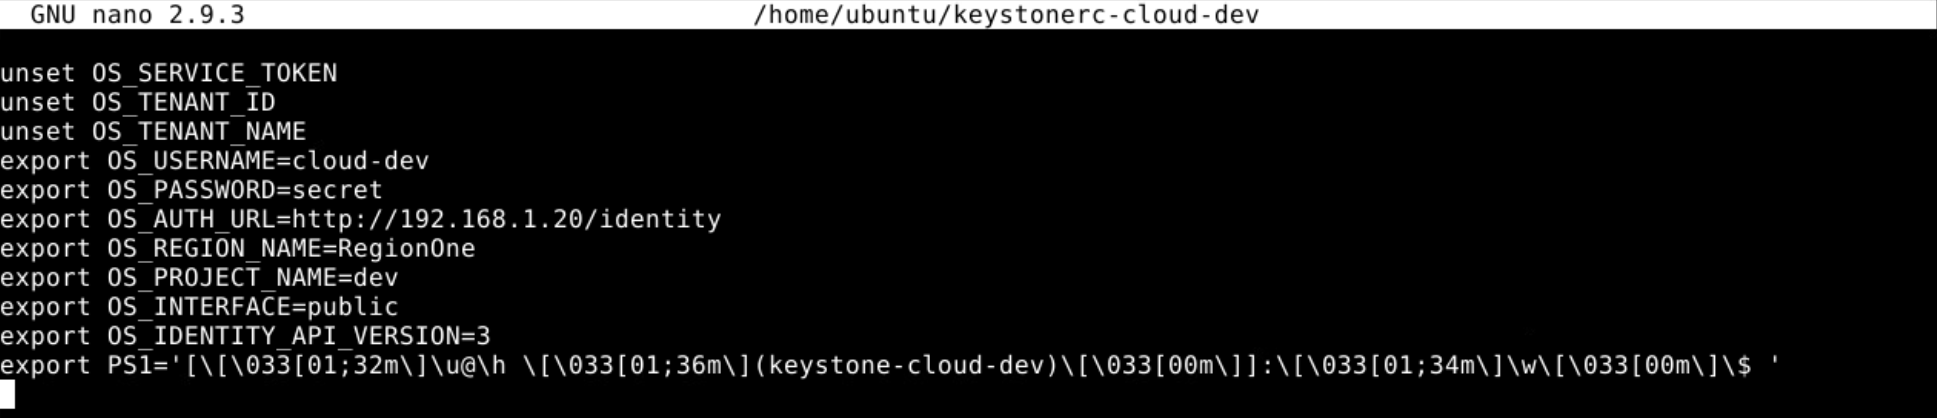
\includegraphics[width=\linewidth]{images/part4/step9.png}
        \end{center}
    \end{labstep}

    \begin{labstep}
        Verify that \textbf{cloud-test3} has the \textbf{member} user role for the \textbf{dev} project.
        \begin{lstlisting}
            [ubuntu@workstation (keystone-admin)]:~$ openstack role assignment list \
            > --user cloud-test3 \
            > --project dev \
            > --names
        \end{lstlisting}

        \begin{center}
            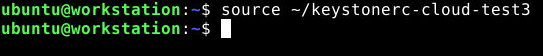
\includegraphics[width=\linewidth]{images/part4/step10.png}
        \end{center}
    \end{labstep}

    \begin{labstep}{it:copy-keystone}
        Copy the existing \textbf{\texttildemid/keystonerc-admin} file to \textbf{\texttildemid/keystonerc-cloud-test3}.
        \begin{lstlisting}
            [ubuntu@workstation (keystone-admin)]:~$ cp ~/keystonerc-admin \
            > ~/keystonerc-cloud-test3
        \end{lstlisting}

        \begin{center}
            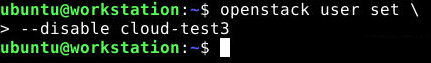
\includegraphics[width=\linewidth]{images/part4/step11.png}
        \end{center}
    \end{labstep}

    \begin{labstep}{it:edit-keystone}
        Edit the \textbf{\texttildemid/keystonerc-cloud-test3} file and change the \textbf{OS\_USERNAME} from \textbf{admin} to \textbf{cloud-test3} and the \textbf{OS\_PROJECT\_NAME} from \textbf{demo} to \textbf{dev}.
        Additionally, change the line beginning with \textbf{export PS1=…} so that \textbf{(keystone-admin)} becomes \textbf{(keystone-cloud-test3)}.
        Modify the file so that the content matches below.
        When you are finished, press \textbf{CTRL+X}, then \textbf{Y} to accept the file changes.
        Press \textbf{Enter} to save and exit \textbf{nano}.
        \begin{lstlisting}
            [ubuntu@workstation (keystone-admin)]:~$ nano ~/keystonerc-cloud-test3
        \end{lstlisting}

        \begin{center}
            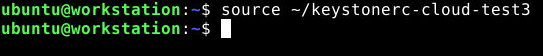
\includegraphics[width=\linewidth]{images/part4/step12.png}
        \end{center}
    \end{labstep}

    \begin{labstep}
        Non-privileged users are limited in the commands they can run and the actions they can perform.
        To demonstrate this, source the \textbf{\texttildemid/keystonerc-cloud-test3} keystone credentials for the \textbf{cloud-test3} user and attempt to list the users.
        You should receive an HTTP 403 (Forbidden) error, which indicates that the user has valid credentials but lacks the privileges to perform the action.
        \begin{lstlisting}
            [ubuntu@workstation (keystone-admin)]:~$ source ~/keystonerc-cloud-test3
            [ubuntu@workstation (keystone-cloud-test3)]:~$ openstack user list
        \end{lstlisting}

        \begin{center}
            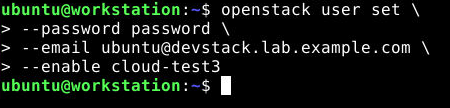
\includegraphics[width=\linewidth]{images/part4/step13.png}
        \end{center}
    \end{labstep}

    \begin{labstep}
        A user with the member role can list and create resources such as flavors and instances.
        As a simple example, list the available flavors.
        \begin{lstlisting}
            [ubuntu@workstation (keystone-cloud-test3)]:~$ openstack flavor list
        \end{lstlisting}

        \begin{center}
            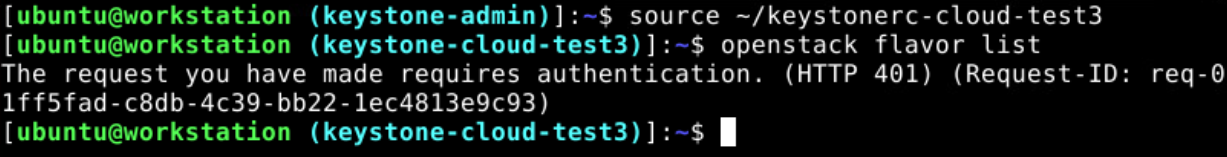
\includegraphics[width=\linewidth]{images/part4/step14.png}
        \end{center}
    \end{labstep}

    \begin{labstep}
        Source the credentials for the \textbf{admin} user, and disable the \textbf{cloud-test3} account.
        \begin{lstlisting}
            [ubuntu@workstation (keystone-cloud-test3)]:~$ source ~/keystonerc-admin
            [ubuntu@workstation (keystone-admin)]:~$ openstack user set \
            > --disable \
            > cloud-test3
        \end{lstlisting}

        \begin{center}
            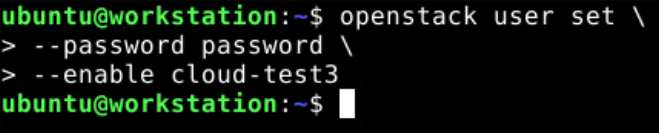
\includegraphics[width=\linewidth]{images/part4/step15.png}
        \end{center}
    \end{labstep}

    \begin{labstep}
        To verify that the \textbf{cloud-test3} account is disabled, source the
        \textbf{\texttildemid/keystonerc-cloud-test3} keystone credentials file for the \textbf{cloud-test3} user.
        Then, try listing the available flavors.
        You should receive an HTTP 401 (Unauthorized) error, which indicates that the user has invalid credentials.
        \begin{lstlisting}
            [ubuntu@workstation (keystone-admin)]:~$ source ~/keystonerc-cloud-test3
            [ubuntu@workstation (keystone-cloud-test3)]:~$ openstack flavor list
        \end{lstlisting}

        \begin{center}
            \includegraphics[width=\linewidth]{images/part4/step16.png}
        \end{center}
    \end{labstep}

    \begin{labstep}
        Source the keystone credentials file of the \textbf{admin} user so that further changes can be made to the \textbf{cloud-test3} user account.
        Then, change the password for the \textbf{cloud-test3} user to \textbf{password}.
        \begin{lstlisting}
            [ubuntu@workstation (keystone-cloud-test3)]:~$ source ~/keystonerc-admin
            [ubuntu@workstation (keystone-admin)]:~$ openstack user set \
            > --password password \
            > cloud-test3
        \end{lstlisting}

        \begin{center}
            \includegraphics[width=\linewidth]{images/part4/step17.png}
        \end{center}
    \end{labstep}

    \begin{labstep}
        Enable the \textbf{cloud-test3} user account.
        \begin{lstlisting}
            [ubuntu@workstation (keystone-admin)]:~$ openstack user set \
            > --enable \
            > cloud-test3
        \end{lstlisting}

        \begin{center}
            \includegraphics[width=\linewidth]{images/part4/step18.png}
        \end{center}
    \end{labstep}

    \begin{tipbox}
        Multiple user settings can be changed with one command.
        For example, this command sets the password and enables the user:
        \begin{lstlisting}
            [ubuntu@workstation (keystone-admin)]:~$ openstack user set \
            > --password password \
            > --enable \
            > cloud-test3
        \end{lstlisting}
    \end{tipbox}

    \begin{labstep}
        In the keystone credentials file for \textbf{cloud-test3}, change the password to \textbf{password}.
        Modify the file so that the content matches below.
        When you are finished, press \textbf{CTRL+X}, then \textbf{Y} to accept the file changes.
        Press \textbf{Enter} to save and exit \textbf{nano}.
        \begin{lstlisting}
            [ubuntu@workstation (keystone-admin)]:~$ nano ~/keystonerc-cloud-test3
        \end{lstlisting}

        \begin{center}
            \includegraphics[width=\linewidth]{images/part4/step19.png}
        \end{center}
    \end{labstep}

    \begin{labstep}
        Source the \textbf{\texttildemid/keystonerc-cloud-test3} keystone credentials file for the
        \textbf{cloud-test3} user.
        \begin{lstlisting}
            [ubuntu@workstation (keystone-admin)]:~$ source ~/keystonerc-cloud-test3
        \end{lstlisting}

        \begin{center}
            \includegraphics[width=\linewidth]{images/part4/step20.png}
        \end{center}
    \end{labstep}

    \begin{labstep}
        Now that the \textbf{cloud-test3} user has been enabled, verify that the \textbf{openstack flavor list} command returns a list of available flavors.
        \begin{lstlisting}
            [ubuntu@workstation (keystone-cloud-test3)]:~$ openstack flavor list
        \end{lstlisting}

        \begin{center}
            \includegraphics[width=\linewidth]{images/part4/step21.png}
        \end{center}
    \end{labstep}

    \begin{labstep}
        Source the keystone credentials file for the \textbf{admin} user.
        \begin{lstlisting}
            [ubuntu@workstation (keystone-cloud-test3)]:~$ source ~/keystonerc-admin
        \end{lstlisting}

        \begin{center}
            \includegraphics[width=\linewidth]{images/part4/step22.png}
        \end{center}
    \end{labstep}

    \begin{labstep}
        Delete the \textbf{cloud-test2} and \textbf{cloud-test3} user accounts since they are no longer needed.
        \begin{lstlisting}
            [ubuntu@workstation (keystone-admin)]:~$ openstack user delete cloud-test2
            [ubuntu@workstation (keystone-admin)]:~$ openstack user delete cloud-test3
        \end{lstlisting}

        \begin{center}
            \includegraphics[width=\linewidth]{images/part4/step23.png}
        \end{center}
    \end{labstep}

    \begin{labstep}
        Verify that the users have been deleted.
        \begin{lstlisting}
            [ubuntu@workstation (keystone-admin)]:~$ openstack user list
        \end{lstlisting}

        \begin{center}
            \includegraphics[width=\linewidth]{images/part4/step24.png}
        \end{center}
    \end{labstep}

    \begin{labstep}
        The lab is now complete.
    \end{labstep}
\end{enumerate}

%%%%%%%%%$
% Appendix
%%%%%%%%%$
\appendix
\section{What Happens if a User Deletes Itself?}
The remainder of the lab will demonstrate the process of creating and using an admin user, and it will explore what happens when a user deletes itself.

\begin{enumerate}
    \begin{labstep}
        Create the user \textbf{cloud-admin2} with the password \textbf{secret}, and make it a member of the
        \textbf{dev} project.
        \begin{lstlisting}
            [ubuntu@workstation (keystone-admin)]:~$ openstack user create \
            > --password secret \
            > --project dev \
            > cloud-admin2
        \end{lstlisting}

        \begin{center}
            \includegraphics[width=\linewidth]{images/appendix/step1.png}
        \end{center}
    \end{labstep}

    \begin{labstep}
        Assign the \textbf{admin} user role to the \textbf{cloud-admin2} user.
        \begin{lstlisting}
            [ubuntu@workstation (keystone-admin)]:~$ openstack role add \
            > --user cloud-admin2 \
            > --project dev \
            > admin
        \end{lstlisting}

        \begin{center}
            \includegraphics[width=\linewidth]{images/appendix/step2.png}
        \end{center}
    \end{labstep}

    \begin{labstep}
        Verify that \textbf{cloud-admin2} has the \textbf{admin} user role for the \textbf{dev} project.
        \begin{lstlisting}
            [ubuntu@workstation (keystone-admin)]:~$ openstack role assignment list \
            > --user cloud-admin2 \
            > --project dev \
            > --names
        \end{lstlisting}

        \begin{center}
            \includegraphics[width=\linewidth]{images/appendix/step3.png}
        \end{center}
    \end{labstep}

    \begin{labstep}
        The \textbf{cloud-admin2} user should now be able to perform admin actions, such as deleting users, in the \textbf{dev} project.
        To act as this user through the command line, first copy the existing \textbf{\texttildemid/keystonerc-admin} file to \textbf{\texttildemid/keystonerc-cloud-admin2}.
        \begin{lstlisting}
            [ubuntu@workstation (keystone-admin)]:~$ cp ~/keystonerc-admin \
            > ~/keystonerc-cloud-admin2
        \end{lstlisting}

        \begin{center}
            \includegraphics[width=\linewidth]{images/appendix/step4.png}
        \end{center}
    \end{labstep}

    \begin{labstep}
        Edit the \textbf{\texttildemid/keystonerc-cloud-admin2} file and change the \textbf{OS\_USERNAME} from \textbf{admin} to \textbf{cloud-admin2} and the \textbf{OS\_PROJECT\_NAME} from \textbf{demo} to \textbf{dev}.
        Additionally, change the line beginning with \textbf{export PS1=…} so that \textbf{(keystone-admin)} becomes \textbf{(keystone-cloud-admin2)}.
        Modify the file so that the content matches below.
        When you are finished, press \textbf{CTRL+X}, then \textbf{Y} to accept the file changes.
        Press \textbf{Enter} to save and exit \textbf{nano}.
        \begin{lstlisting}
            [ubuntu@workstation (keystone-admin)]:~$ nano ~/keystonerc-cloud-admin2
        \end{lstlisting}

        \begin{center}
            \includegraphics[width=\linewidth]{images/appendix/step5.png}
        \end{center}
    \end{labstep}

    \begin{labstep}
        Source the \textbf{\texttildemid/keystonerc-cloud-admin2} keystone credentials file for the \textbf{cloud-admin2} user.
        \begin{lstlisting}
            [ubuntu@workstation (keystone-admin)]:~$ source ~/keystonerc-cloud-admin2
        \end{lstlisting}

        \begin{center}
            \includegraphics[width=\linewidth]{images/appendix/step6.png}
        \end{center}
    \end{labstep}

    \begin{labstep}
        List the current OpenStack users to see the list of users that can be deleted.
        \begin{lstlisting}
            [ubuntu@workstation (keystone-cloud-admin2)]:~$ openstack user list
        \end{lstlisting}

        \begin{center}
            \includegraphics[width=\linewidth]{images/appendix/step7.png}
        \end{center}
    \end{labstep}

    \begin{labstep}
        If a user has sufficient privileges, it can delete itself.
        To test this, delete the \textbf{cloud-admin2} user, the current user whose keystone credentials are being used.
        \begin{lstlisting}
            [ubuntu@workstation (keystone-cloud-admin2)]:~$ openstack user delete \
            > cloud-admin2
        \end{lstlisting}

        \begin{center}
            \includegraphics[width=\linewidth]{images/appendix/step8.png}
        \end{center}
    \end{labstep}

    \begin{labstep}
        Since the \textbf{cloud-admin2} user has been deleted, the keystone credentials no longer authenticates the user.
        Verify this by attempting to list the OpenStack users.
        You should receive an HTTP 401 (Unauthorized) error, which indicates that the user has invalid credentials.
        \begin{lstlisting}
            [ubuntu@workstation (keystone-cloud-admin2)]:~$ openstack user list
        \end{lstlisting}

        \begin{center}
            \includegraphics[width=\linewidth]{images/appendix/step9.png}
        \end{center}
    \end{labstep}

    \begin{labstep}
        Source the \textbf{\texttildemid/keystonerc-admin} keystone credentials file for the \textbf{admin} user.
        \begin{lstlisting}
            [ubuntu@workstation (keystone-cloud-admin2)]:~$ source ~/keystonerc-admin
        \end{lstlisting}

        \begin{center}
            \includegraphics[width=\linewidth]{images/appendix/step10.png}
        \end{center}
    \end{labstep}

    \begin{labstep}
        Verify that the \textbf{cloud-admin2} user has been deleted.
        \begin{lstlisting}
            [ubuntu@workstation (keystone-admin)]:~$ openstack user list
        \end{lstlisting}

        \begin{center}
            \includegraphics[width=\linewidth]{images/appendix/step11.png}
        \end{center}
    \end{labstep}

\end{enumerate}
\end{document}
